\documentclass[journal]{IEEEtran}

% --- CORE & MATH PACKAGES ---
\usepackage{cite}
\usepackage{amsmath,amssymb,amsfonts}
\usepackage{textcomp}
\usepackage{graphicx}
\usepackage{tabularx}

% --- FONT CONFIGURATION ---
\usepackage{newtxtext}
\usepackage{newtxmath}

% --- ALGORITHM ENVIRONMENT SETUP (algorithm2e) ---
% Using algorithm2e for a modern algorithm style. This has NO conflict.
\usepackage[ruled,vlined,linesnumbered]{algorithm2e}

% --- UTILITY PACKAGES ---
\usepackage{float}
\usepackage{caption}
\usepackage{subcaption}

% graph making
% --- 图表与子图包 ---

% --- TikZ 绘图包 (请将这些放在导言区) ---
\usepackage{tikz}
\usetikzlibrary{
    shapes.geometric,
    shapes,
    arrows.meta,
    positioning,
    fit,
    calc
}
% after we removed the conflicting 'amsthm' package.
\newtheorem{theorem}{Theorem}
\newtheorem{proposition}{Proposition}
\newtheorem{lemma}{Lemma}
\newtheorem{corollary}{Corollary}
\newtheorem{remark}{Remark}
% The 'proof' environment is typically built-in with the IEEEtran class,




\begin{document}

% --- TITLE ---
\title{System Relaxation Algorithm (SRA): An Interpretable, Adaptive Approach to Dispersing Network Structural Stress}


% --- AUTHOR INFORMATION ---
% TODO: Please fill in your author details here.
% Use \thanks for affiliations and funding information.
\author{Zhiyuan~Ren,~\IEEEmembership{Member,~IEEE},
        Yutao~Liu,
        Wenchi~Cheng,~\IEEEmembership{Senior~Member,~IEEE},
        and Mingxuan Lu%
\thanks{This work was supported in part by the National Key Research and Development Program of China under Grant No. 2024YFE0200300.}%
\thanks{Zhiyuan Ren, Yutao Liu, and Wenchi Cheng are with the School of Telecommunications Engineering, Xidian University, Xi'an 710071, China.}%
\thanks{Kun Yang is with the School of Computer Science and Electronic Engineering, University of Essex, Colchester CO4 3SQ, U.K.}%
\thanks{Corresponding author: Zhiyuan Ren (zyren@xidian.edu.cn).}%
}



% --- The paper headers (optional) ---
\markboth{IEEE TRANSACTIONS ON CONTROL OF NETWORK SYSTEMS, VOL. XX, NO. X, MONTH 202X}%
{Author \MakeLowercase{\textit{et al.}}: System Relaxation Algorithm (SRA)}


% --- GENERATE THE TITLE ---
\maketitle


% --- ABSTRACT ---
\begin{abstract}
Prevailing network control strategies, often reliant on static, shortest-path logic, lack an intrinsic mechanism for managing structural stress. This design oversight leads to catastrophic "stress concentration" on critical nodes, causing failures due to local congestion long before the network reaches its theoretical capacity. This paper introduces the System Relaxation Algorithm (SRA), a new control paradigm inspired by physical relaxation that guides a network's resource utilization toward an emergent equilibrium of load balance. At its core, SRA is an interpretable, 'white-box' dynamical system that reframes the problem: not as one of pathfinding, but of system-level stress control. It uses a theoretically verifiable leaky integrator to couple a node's transit cost---the control signal---with its historically accumulated structural stress, thereby steering the network's evolution. Crucially, SRA's behavior is profoundly topology-dependent: in heterogeneous networks with significant bottlenecks (e.g., Barabási-Albert networks), it functions as a proactive performance optimizer, reducing peak centrality by over 80\% and increasing high-load throughput by more than 45\%. Conversely, in more homogeneous topologies where such bottlenecks are less pronounced, its objective intelligently shifts from performance maximization to resilience enhancement, substantially increasing robustness against structural damage. Theoretically, we rigorously prove its global convergence and practical stability based on the theory of non-smooth dynamical systems. Ultimately, SRA provides a predictable paradigm for a new class of network governance strategies. By actively managing structural stress, it enables an intelligent trade-off between performance and resilience, with significant implications for data centers, tactical ad-hoc networks, and beyond.
\end{abstract}

% --- KEYWORDS ---
\begin{IEEEkeywords}
Network control, stress-aware governance, network resilience, self-organizing systems, load balancing, non-smooth dynamical systems, stability analysis.
\end{IEEEkeywords}


% --- Body of the paper starts here ---
% --- SECTION I: Introduction ---
\section{Introduction}
\label{sec:introduction}

\IEEEPARstart{I}{n} both nature and engineering, a ubiquitous phenomenon is the spontaneous evolution of complex systems from high-energy, high-stress non-equilibrium states toward more stable, orderly equilibria. This process of "relaxation," observed from crystal growth to the annealing of metals, enables a system to disperse internal stress by rearranging its microscopic structures to achieve a macroscopically more robust state. However, prevailing network control paradigms, and particularly the design of their routing protocols, lack such an intrinsic stress regulation mechanism.

As a quintessential complex system, a communication network's performance is profoundly influenced by the distribution of "stress" within its topology. We define this "stress" as a measure of imbalanced load concentration, which can be formalized using the network science metric of \textbf{Betweenness Centrality (BC)}. A high BC value for a node signifies its critical role as a topological "traffic hub" and thus a point of structural vulnerability. This metric transforms an intuitive concept into a measurable quantity, allowing us to identify and analyze the endemic problem of extreme \textbf{stress concentration} on a few critical nodes.

This high-stress state, a form of "kinetically constrained" equilibrium, manifests as two measurable symptoms. Structurally, it appears as an extreme concentration of Betweenness Centrality on a few hub nodes, forming "stress singularities" that make the topology fragile and vulnerable to cascading failures. Performatively, it leads to premature capacity saturation, where these bottleneck hubs cause massive packet loss and soaring latency long before the network's physical capacity is reached. Fig.~\ref{fig:intro_scenario} provides a conceptual illustration of this core problem and our proposed control paradigm. As depicted in Fig.~\ref{fig:intro_before}, the conventional paradigm's focus on shortest paths naturally creates these stress points. In contrast, the goal of the SRA paradigm, shown in Fig.~\ref{fig:intro_after}, is to proactively disperse this stress, guiding the network toward a more robust and "relaxed" state.

\begin{figure}[t!]
    \centering
    % ---- (a) Before SRA ----
    \begin{subfigure}[b]{0.47\columnwidth} % <-- 宽度设为 0.47
        \centering
        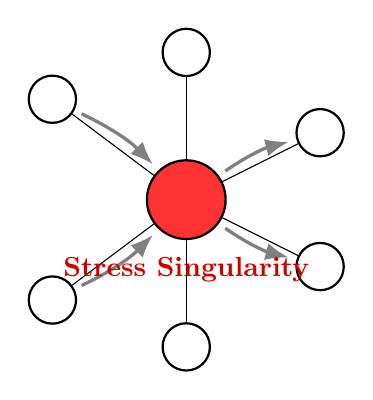
\begin{tikzpicture}[scale=0.85] % <-- 图形缩放为 85%
            \tikzstyle{node}=[circle, draw, thick, minimum size=6mm]
            \tikzstyle{hub}=[node, fill=red!80, minimum size=10mm]
            \tikzstyle{flow}=[-Latex, gray, thick, shorten <=1mm, shorten >=1mm]
            % Nodes
            \node[hub] (H) at (0,0) {};
            \node[node] (N1) at (2,1) {};
            \node[node] (N2) at (2,-1) {};
            \node[node] (N3) at (-2,1.5) {};
            \node[node] (N4) at (-2,-1.5) {};
            \node[node] (P1) at (0, 2.2) {};
            \node[node] (P2) at (0, -2.2) {};
            % Edges
            \draw (H) -- (N1); \draw (H) -- (N2);
            \draw (H) -- (N3); \draw (H) -- (N4);
            \draw (H) -- (P1); \draw (H) -- (P2);
            % Traffic Flows
            \draw[flow, line width=1.2pt] (N3) to [bend left=10] (H);
            \draw[flow, line width=1.2pt] (N4) to [bend right=10] (H);
            \draw[flow, line width=1.2pt] (H) to [bend left=10] (N1);
            \draw[flow, line width=1.2pt] (H) to [bend right=10] (N2);
            \node[below=0.1cm of H, text=red!80!black, font=\bfseries] {Stress Singularity};
        \end{tikzpicture}
        \caption{Conventional Paradigm: Stress Concentration}
        \label{fig:intro_before}
    \end{subfigure}
    \hfill
    % ---- (b) After SRA ----
    \begin{subfigure}[b]{0.47\columnwidth} % <-- 宽度设为 0.47
        \centering
        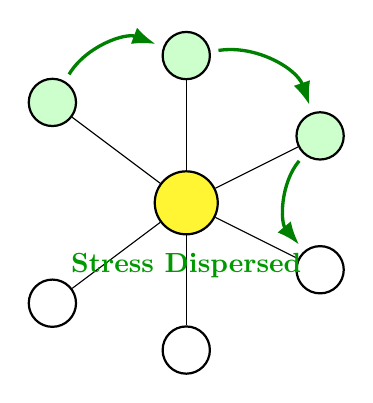
\begin{tikzpicture}[scale=0.85] % <-- 图形缩放为 85%
            \tikzstyle{node}=[circle, draw, thick, minimum size=6mm]
            \tikzstyle{hub}=[node, fill=yellow!80, minimum size=8mm]
            \tikzstyle{periph}=[node, fill=green!20]
            \tikzstyle{flow}=[-Latex, green!50!black, thick, shorten <=1mm, shorten >=1mm]
            % Nodes
            \node[hub] (H) at (0,0) {};
            \node[periph] (N1) at (2,1) {};
            \node[node] (N2) at (2,-1) {};
            \node[periph] (N3) at (-2,1.5) {};
            \node[node] (N4) at (-2,-1.5) {};
            \node[periph] (P1) at (0, 2.2) {};
            \node[node] (P2) at (0, -2.2) {};
            % Edges
            \draw (H) -- (N1); \draw (H) -- (N2);
            \draw (H) -- (N3); \draw (H) -- (N4);
            \draw (H) -- (P1); \draw (H) -- (P2);
            % Traffic Flows
            \draw[flow, line width=1.2pt] (N3) to [bend left=40] (P1);
            \draw[flow, line width=1.2pt] (P1) to [bend left=40] (N1);
            \draw[flow, line width=1.2pt] (N1) to [bend right=40] (N2);
            \node[below=0.1cm of H, text=green!60!black, font=\bfseries] {Stress Dispersed};
        \end{tikzpicture}
        \caption{SRA Control Paradigm: System Relaxation}
        \label{fig:intro_after}
    \end{subfigure}
    
    \caption{Conceptual illustration of the core problem and the proposed SRA paradigm. SRA mitigates the "stress concentration" inherent in conventional network control by guiding the system to a "relaxed" state of balanced load.}
    \label{fig:intro_scenario}
\end{figure}

The root of this fragility lies in the limitations of the prevailing network control paradigm. Static, shortest-path protocols are oblivious to the emergent stress distribution, perpetually confining the network to a suboptimal state. While subsequent adaptive routing methods attempt to mitigate the symptoms by reacting to transient, traffic-driven metrics such as queue lengths, they fail to address the underlying structural cause. Their common flaw is a narrow focus on \textit{pathfinding} within a given cost landscape, rather than on \textit{controlling the landscape itself}.

This paper proposes a paradigm shift from reactive pathfinding to proactive stress control. We introduce the System Relaxation Algorithm (SRA) not as another routing algorithm, but as a model-driven control system designed to manage this intrinsic structural stress. Furthermore, this control paradigm is perfectly aligned with modern architectures like Software-Defined Networking (SDN). An SDN controller provides the ideal platform for SRA's implementation: it naturally possesses the global network view required for stress calculation and offers direct mechanisms to enforce the resulting policies on the data plane. SRA, therefore, represents a high-level control application that equips SDN with the intelligence to translate its centralized visibility into proactive structural resilience.

Our main contributions are organized around three central axes:

\begin{enumerate}
    \item \textbf{A Novel Control-Theoretic Model:} We introduce "system relaxation" as a new control paradigm for network governance. This framework is the first to formalize endemic structural stress, quantified via betweenness centrality, as a controllable state variable within a fully interpretable, "white-box" dynamical system.

    \item \textbf{Rigorous Analysis of Discontinuous Dynamics:} To the best of our knowledge, this is the first work to rigorously model the discrete, discontinuous path switching in network control as a non-smooth dynamical system. By applying specialized tools like piecewise Lyapunov functions, we provide formal proofs of stability, effectively managing the complex dynamics akin to phase transitions in other complex systems.

    \item \textbf{Demonstrable Enhancement of Structural Robustness:} Through comprehensive simulations, we demonstrate that this control mechanism guides the network to self-organize into a verifiably more robust state. The outcome is not merely performance optimization but a fundamental enhancement of the network's resilience to both structural damage and dynamic congestion, achieved via an intelligent, topology-aware trade-off.
\end{enumerate}

The remainder of this paper is organized as follows. Section~\ref{sec:related_work} reviews related work. Section~\ref{sec:model} details our theoretical model and its analysis. Section~\ref{sec:simulation} presents the simulation results. Section~\ref{sec:discussion} provides an in-depth discussion, and Section~\ref{sec:conclusion} concludes the paper.


\section{Related Work}
\label{sec:related_work}

The design of routing protocols for dynamic networks is a well-established field, traditionally categorized into proactive, reactive, and hybrid approaches. However, the rise of structurally complex and unpredictable networks, such as tactical ad-hoc and Internet of Things (IoT) networks, has exposed the limitations of these classic paradigms, particularly their inability to handle the "stress concentration" problem. This has spurred research into two primary advanced methodologies: load-aware routing and AI-driven routing. SRA, as proposed in this paper, represents a third, model-driven approach that integrates concepts from both while maintaining full interpretability. Table~\ref{tab:related_work_comparison} provides a comparative positioning of SRA against these paradigms.

\subsection{Traditional Load-Aware Routing}
Load-aware routing protocols dynamically adjust paths based on real-time network state metrics. These metrics often include local information such as node queue lengths \cite{14}, channel busyness \cite{11}, or composite path load metrics \cite{4}. For instance, the ALR protocol proposed by S and M \cite{11} uses a composite metric of queue length and packet transmission success rate to select paths. Similarly, the CRADLE protocol by Macabale et al. \cite{14} leverages queue occupancy and channel state information for path selection in wireless mesh networks. The LIRP protocol by Tao et al. \cite{4} employs a cost function based on link quality and queue length. While effective at mitigating immediate, localized congestion, these methods often rely on heuristic rules and lack a global perspective on network structure. They primarily focus on state-aware path selection rather than fundamentally reshaping the underlying "cost landscape" of the network based on its structural properties, a key differentiator of our SRA framework.

\subsection{Static Centrality-Based Routing Optimization}
Centrality metrics, which quantify the structural importance of nodes, have been widely used to inform routing decisions. While some studies have explored physical layering \cite{1} or closeness centrality \cite{13}, betweenness centrality (BC) \cite{9, 12} is the most common metric for identifying structural bottlenecks. Several studies have proposed static or quasi-static methods that leverage BC. For example, Ahmed et al. \cite{7} and Ma and Yang \cite{18} used pre-calculated BC to optimize routing paths and flow table storage, respectively. Upadhyay and Singh \cite{6} attempted to use a genetic algorithm to find a single, static network configuration that minimizes the variance of BC. However, calculating BC is computationally intensive \cite{8}, and recent efforts have focused on distributed computation methods \cite{17, 19}. The primary limitation of these approaches is their static or infrequently updated nature, which struggles to adapt to the rapid, dynamic changes in network topology and traffic that our SRA framework is designed to handle.

\subsection{AI-Driven Adaptive Routing}
Modern AI techniques, particularly machine learning and reinforcement learning, have been applied to create highly adaptive routing protocols. These methods can be broadly categorized as either heuristic optimization or reinforcement learning-based. Heuristic approaches like Genetic Algorithms (GA) \cite{2} and Particle Swarm Optimization (PSO) \cite{10, 16} can search for optimal routing policies but often require significant computational resources.

Reinforcement learning (RL) offers a more online, adaptive approach. Classical Q-learning algorithms \cite{15} have been used to allow nodes to learn optimal next-hops based on local rewards. More advanced methods now combine Graph Neural Networks (GNNs) with Deep Reinforcement Learning (DRL) \cite{3, 5} to learn complex relationships between network topology and traffic state for more sophisticated path selection. While powerful, these AI-driven methods often function as "black boxes," making their behavior difficult to predict, interpret, or formally verify. This lack of interpretability is a significant barrier to their deployment in mission-critical systems. In contrast, SRA is a fully model-driven, "white-box" framework whose behavior is governed by a clear, mathematically tractable dynamical system, a key advantage for mission-critical applications.

\subsection{Positioning of Our Work}
\label{subsec:positioning}

In summary, the novelty of the SRA framework lies in its unique synthesis and transcendence of the ideas from the aforementioned technical routes. It fundamentally differs from conventional methods by being \textbf{structural and proactive} rather than symptomatic and reactive, naturally suppressing oscillations through an integral controller with memory. It advances beyond static centrality optimization by being \textbf{dynamic and closed-loop}, revolutionizing centrality from a static analysis tool into a real-time control signal. Finally, it provides a crucial alternative to AI-based routing by being \textbf{mechanistically interpretable}, offering the predictability and reliability essential for core network protocols, a stark contrast to data-driven "black boxes." These fundamental distinctions are summarized in Table~\ref{tab:related_work_comparison}.

Therefore, the uniqueness and core contribution of SRA lie not in any single technical component, but in its success in building a solid theoretical bridge between three major knowledge domains: it employs centrality measures from \textbf{network science} as the sensing signal, utilizes an integrator from \textbf{control theory} as the actuation engine, and finally, applies the theory of \textbf{non-smooth dynamical systems} to provide rigorous mathematical guarantees for its stable operation. It is this systematic, cross-disciplinary integration that distinguishes SRA from existing methods and offers a completely new, model-driven paradigm for resilient network design.


\begin{table}[t!]
\centering
\caption{Comparative Positioning of SRA against Existing Routing Paradigms}
\label{tab:related_work_comparison}
\renewcommand{\arraystretch}{1.2}
\small
\begin{tabularx}{\columnwidth}{|l|X|X|X|}
\hline
\textbf{Feature} & \textbf{Traditional Load-Aware} & \textbf{AI-Driven} & \textbf{SRA (This Work)} \\
\hline \hline
\textbf{Sensing Object} & Real-time traffic state (e.g., queue lengths) & Traffic patterns \& Topology features & \textbf{Accumulated structural stress} \\
\hline
\textbf{Timescale} & Instantaneous / Short-term & Short to Medium-term & \textbf{Long-term structural equilibrium} \\
\hline
Primary Goal & Mitigate local, transient congestion & Maximize performance metrics (e.g., throughput) & Disperse endemic structural stress \\
\hline
Core Method & Heuristic cost functions & Black-box learning (e.g., RL, GNN) & Model-driven dynamical system \\
\hline
Interpretability & High & Low & High \\
\hline
\end{tabularx}
\end{table}

% --- SECTION III: Theoretical Model and Methods ---
\section{Theoretical Model and Methods}
\label{sec:model}

\begin{table}[t!]
\centering
\caption{Table of Principal Notations}
\label{tab:notations}
\renewcommand{\arraystretch}{1.2} % 增加行高
\begin{tabular}{c l}
\hline
\hline
\textbf{Symbol} & \textbf{Definition / Description} \\
\hline
\multicolumn{2}{l}{\textit{A. Network and Control System Parameters}} \\
$G, V, E, N$ & Network graph, sets of nodes and edges, num. of nodes. \\
$S \in \mathbb{R}^N_+$ & State vector representing accumulated structural pressure. \\
$\kappa \in \mathbb{R}^N_+$ & Unnormalized betweenness centrality vector (load). \\
$C \in \mathbb{R}^N_+$ & Node transit cost vector (control output). \\
$\mu_i$ & Service rate (processing capacity) of node $i$. \\
$\alpha \in (0,1)$ & Learning rate in the leaky integrator. \\
$\beta_I > 0$ & Pressure-to-cost conversion factor. \\
$T_d \ge 1$ & Minimum dwell time between path-switching events. \\
$K_{\max}, \varepsilon$ & Max iterations and stopping threshold for Algorithm 1. \\
\hline
\multicolumn{2}{l}{\textit{B. Performance and Analysis Metrics}} \\
$\kappa_{\max}$ & Maximum value in the vector $\kappa$ (peak centrality). \\
$\rho_{\max}$ & Network capacity (maximum sustainable load). \\
$c \in [0,1]^N$ & Max-normalized centrality vector, used in state updates. \\
$V(S)$ & Piecewise Lyapunov function (system energy). \\
$\{v_\ell\}$ & Finite set of all possible constant vectors for $c$. \\
$\bar\Delta$ & Diameter of the set $\{v_\ell\}$ under the $\ell_2$-norm. \\
$\gamma, \tilde\Delta$ & Recurrence parameters, $\gamma=1-\alpha$, $\tilde\Delta=\bar\Delta^2/\alpha$. \\
$L(\kappa)$ & Robust lower bound on network capacity, $L(\kappa)=\mu_{\min}/\kappa_{\max}$. \\
\hline
\hline
\end{tabular}
\end{table}

Having established the conceptual foundation of SRA, this Section delves into its theoretical core. The primary challenge in designing any adaptive routing protocol is not merely achieving responsiveness, but ensuring \textbf{provable stability}; many naive, reactive approaches ultimately collapse into destructive oscillations. To overcome this, we move beyond simple heuristics and formally construct SRA as a \textbf{discrete-time, non-smooth dynamical system}. This control-theoretic approach is essential, as it allows us to precisely model the complex interplay between the continuous evolution of node costs and the discrete "switching" of routing paths.

This section provides a systematic exposition of this system. We begin by defining the network model and the centrality-based state variables that quantify "structural stress." We then detail the core evolution rule—the leaky integrator—that provides the system with both memory and damping. The culmination of this Section is a rigorous proof of SRA's global convergence and practical stability, for which we employ the powerful tools of piecewise Lyapunov functions and discrete-time inclusion theory. This analysis provides the solid theoretical cornerstone that guarantees SRA's predictable and reliable behavior, bridging the gap from an algorithmic concept to a robust engineering solution.

\subsection{Network Model and Load Metric}

We model the infrastructure network as an undirected graph $G=(V,E)$, where $V$ is the set of nodes, $E$ is the set of edges, and the total number of nodes is $N=|V|$. Throughout the iterative process of SRA, the path lengths in the network are calculated based on a dynamically evolving node cost vector $C \in \mathbb{R}^N_+$. Specifically, the cost of any given path $P$ is defined as the sum of the transit costs of all nodes comprising it, i.e., $d(P) = \sum_{v \in P} C_v$. Standard shortest-path algorithms, such as Dijkstra's, are then executed on the graph where the objective is to minimize this cumulative node-based path cost.
Throughout this paper, we assume the network $G$ is connected and has at least three nodes ($N \ge 3$).

To quantify the load concentration effect induced by the network topology and the current cost distribution, this paper employs \textbf{Betweenness Centrality (BC)} as the core metric. Given a state $S$ and its corresponding node costs $C(S)$, the (unnormalized) betweenness centrality of a node i is defined as the total number of all-pairs shortest paths, calculated using $C(S)$ as node weights, that pass through node i:
\begin{equation}
    \label{eq:bc_definition}
    \kappa_i(S) = \sum_{s\neq i\neq t\in V} \frac{\sigma^{\,C(S)}_{st}(i)}{\sigma^{\,C(S)}_{st}}
\end{equation}
where $\sigma^{\,C(S)}_{st}$ is the total number of shortest paths from node $s$ to node $t$ under the cost metric $C(S)$, and $\sigma^{\,C(S)}_{st}(i)$ is the number of those paths that pass through node $i$. 
% --- INSERT THE NEW CLARIFICATION PARAGRAPH HERE ---
\textbf{It is critical to note that while the term within the summation, $\sigma^{\,C(S)}_{st}(i)/\sigma^{\,C(S)}_{st}$, represents a proportion for a single source-destination pair, the total centrality $\kappa_i(S)$ is the sum of these proportions over all distinct pairs. Consequently, $\kappa_i(S)$ is an unbounded, positive real number that reflects the absolute magnitude of a node's bridging role, and its value can significantly exceed 1.}

Therefore, to ensure the boundedness of the state variables in our dynamical system, we employ the centrality vector after max-value normalization in the algorithm's update steps:
\begin{equation}
    \label{eq:bc_normalization}
    \mathrm{norm}(\kappa(S)) :=
    \begin{cases}
    \displaystyle \frac{\kappa(S)}{\max_{j}\kappa_j(S)}, & \text{if } \max_j \kappa_j(S) > 0,\\[6pt]
    \mathbf{0}, & \text{otherwise.}
    \end{cases}
\end{equation}
Consequently, the value of $\mathrm{norm}(\kappa(S))$ is always confined within the unit hypercube $[0,1]^N$. A key corollary is that, given that the graph $G$ has a finite number of nodes and edges, and assuming a \textbf{globally fixed and deterministic tie-breaking rule} for shortest paths with equal costs, the set of all possible shortest path combinations across the network is finite. Therefore, the set of all possible values for $\mathrm{norm}(\kappa(S))$, which is determined by these path combinations, must also constitute a finite set of constant vectors. This property is a cornerstone of the subsequent convergence analysis.

\subsection{SRA: Core Mechanism and Algorithm Implementation}
\label{subsec:sra_mechanism}

% --- 这是 Fig. 2 的完整、修正版代码 ---
\begin{figure*}[hbtp]
    \centering
    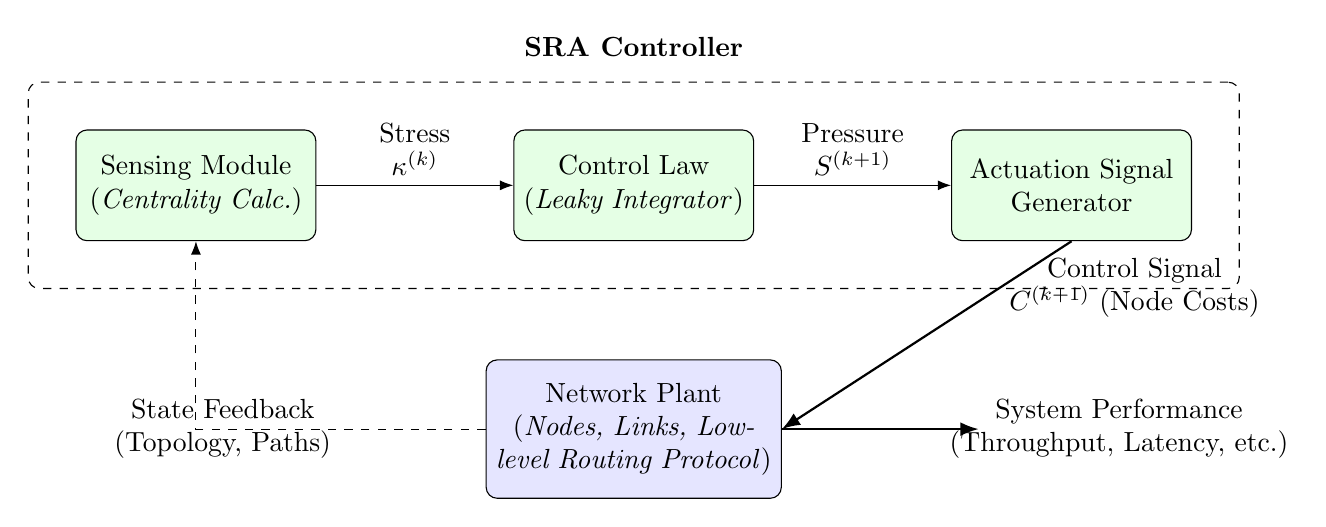
\begin{tikzpicture}[
        auto,
        node distance=1.5cm and 2.5cm,
        plant/.style={rectangle, draw, fill=blue!10, text width=10em, text centered, rounded corners, minimum height=5em},
        module/.style={rectangle, draw, fill=green!10, rounded corners, text width=8em, text centered, minimum height=4em}, % <-- 为内部模块定义了清晰的样式
        line/.style={draw, -{Latex}},
        signal/.style={draw, -{Latex}, thick},
        feedback/.style={draw, -{Latex}, dashed}
    ]
    
    % SRA Controller's Internal Modules (应用了新的 'module' 样式)
    \node [module] (sensing) {Sensing Module \\ (\textit{Centrality Calc.})};
    \node [module, right=of sensing] (law) {Control Law \\ (\textit{Leaky Integrator})};
    \node [module, right=of law] (actuation) {Actuation Signal Generator};

    % Network Plant
    \node [plant, below=of law] (plant) {Network Plant \\ (\textit{Nodes, Links, Low-level Routing Protocol})};
    
    % Dashed container for the SRA controller
    \node [draw, rounded corners, fit=(sensing) (law) (actuation), label={[yshift=0.2cm]above:\textbf{SRA Controller}}, inner sep=0.6cm, dashed] (controller_box) {};

    % Connections
    \path [signal] (actuation.south) -- node [right, pos=0.25, align=center] {Control Signal \\ $C^{(k+1)}$ (Node Costs)} (plant.east);
    \path [feedback] (plant.west) -| node [left, pos=0.25, align=center] {State Feedback \\ (Topology, Paths)} (sensing.south);
    
    % Internal Controller Connections
    \path [line] (sensing.east) -- node [above, align=center] {Stress \\ $\kappa^{(k)}$} (law.west);
    \path [line] (law.east) -- node [above, align=center] {Pressure \\ $S^{(k+1)}$} (actuation.west);

    % System Performance Output
    \coordinate[right=of plant] (output_coord);
    \path [signal] (plant.east) -- node [right, pos=0.8, align=center] {System Performance \\ (Throughput, Latency, etc.)} (output_coord);

    \end{tikzpicture}
    \caption{The architecture of the SRA as a closed-loop control system. The SRA controller acts as a supervisory layer that governs the underlying network plant by dynamically adjusting the cost landscape.}
    \label{fig:sra_architecture}
\end{figure*}


Having defined the network model and the load metric, this section details the core of the SRA framework: its dynamic cost evolution rule. We present this not merely as an algorithm, but as the formal design of a dynamical system's control law. The overall architecture of this closed-loop system is depicted in Fig.~\ref{fig:sra_architecture}, illustrating the clear separation between the SRA controller and the underlying network plant it governs.

\subsubsection{Dynamic Cost Evolution Mechanism}
SRA's core innovation is its conceptualization of the network as a dynamically evolving "cost landscape." A naive feedback mechanism would be a simple proportional (P) controller, making a node's cost proportional to its current centrality ($\kappa_i$). However, such a "memoryless" mechanism is fundamentally unstable, as it inevitably leads to violent and persistent oscillations, failing to converge.

To ensure stability, SRA's design must incorporate memory, leading to an Integral (I) control structure. We conceptualize this using a physical analogy: a sealed chamber with a release valve. The node's centrality acts as a gas inflow, while a core \textbf{state vector}, which we term the "accumulated pressure" $S \in \mathbb{R}^N_+$, represents the internal pressure that builds up while slowly decaying. This process is formalized by the following discrete-time \textbf{state transition equation}:
\begin{equation}
    \label{eq:pressure_update}
    S_i^{(k+1)} = (1 - \alpha) S_i^{(k)} + \alpha \cdot \mathrm{norm}(\kappa_i^{(k)})
\end{equation}
where $k$ is the iteration step and $\alpha \in (0,1)$ is the learning rate. This equation is, in essence, a \textbf{leaky integrator} (or a first-order low-pass filter). The $(1-\alpha)$ term provides a critical \textbf{damping} effect, ensuring the stability of the integration process, while the $\alpha$ term controls the rate at which the system tracks the current load signal.

The node transit cost $C$, which can be seen as the system's \textbf{output}, is then defined as an affine function of the state:
\begin{equation}
    \label{eq:cost_update}
    C_i^{(k+1)} = 1 + \beta_I \cdot S_i^{(k+1)}
\end{equation}
where $1$ is a base cost and $\beta_I > 0$ is the "pressure-to-cost" conversion factor. By defining the cost as a function of the system's historical state ($S$), SRA makes stable and proactive path selection decisions.

\begin{figure}[hbtp]
    \centering
    \resizebox{\columnwidth}{!}{% <-- 在这里开始 resizebox
        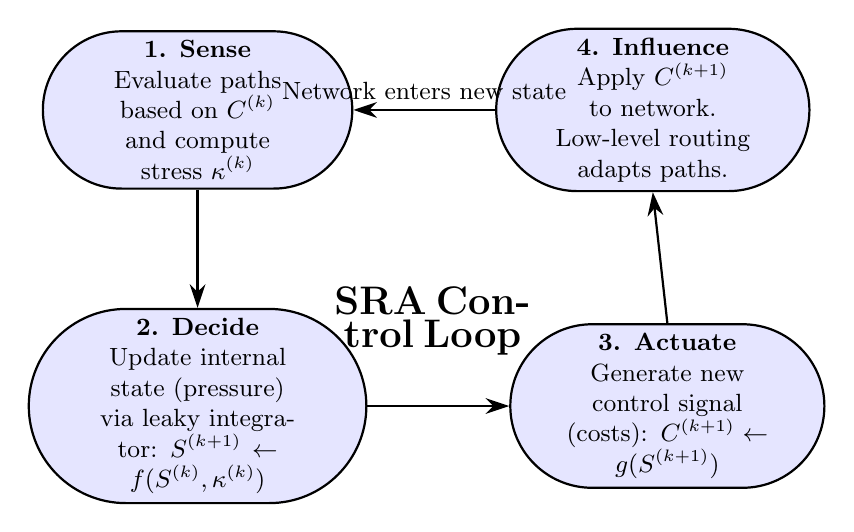
\begin{tikzpicture}[
            node distance=1.5cm and 1.8cm,
            process/.style={
                rounded rectangle, 
                draw, 
                fill=blue!10, 
                text width=7.5em,
                text centered, 
                minimum height=4em,
                thick,
                font=\small
            },
            arrow/.style={
                -{Stealth[length=3mm, width=2mm]},
                thick
            }
        ]
        
        % Nodes in the cycle
        \node[process] (sense) {\textbf{1. Sense} \\ Evaluate paths based on $C^{(k)}$ and compute stress $\kappa^{(k)}$};
        \node[process, below=of sense] (decide) {\textbf{2. Decide} \\ Update internal state (pressure) via leaky integrator: $S^{(k+1)} \leftarrow f(S^{(k)}, \kappa^{(k)})$};
        \node[process, right=of decide] (actuate) {\textbf{3. Actuate} \\ Generate new control signal (costs): $C^{(k+1)} \leftarrow g(S^{(k+1)})$};
        \node[process, right=of sense] (influence) {\textbf{4. Influence} \\ Apply $C^{(k+1)}$ to network. Low-level routing adapts paths.};
        
        % Arrows connecting the nodes
        \draw[arrow] (sense.south) -- (decide.north);
        \draw[arrow] (decide.east) -- (actuate.west);
        \draw[arrow] (actuate.north) -- (influence.south);
        \draw[arrow] (influence.west) -- node[above, font=\small] {Network enters new state} (sense.east);
        
        % Add a title inside the loop
        \node[text width=8em, text centered] at ($(sense)!0.5!(actuate) + (0, -0.8)$) {\Large \textbf{SRA Control Loop}};
    
        \end{tikzpicture}
    } % <-- 在这里结束 resizebox
    \caption{The iterative workflow of the SRA control loop, illustrating the four key phases of sensing, decision-making, actuation, and system influence that drive the network toward a state of dispersed structural stress.}
    \label{fig:sra_workflow}
\end{figure}

\subsubsection{Algorithm Implementation}
The complete iterative process of SRA is precisely described in Algorithm~\ref{alg:sra}, and its cyclical, four-phase workflow is visualized in Fig.~\ref{fig:sra_workflow}. Step 5 of the algorithm introduces a key tunable parameter, the minimum dwell time $T_d$. This parameter is not merely a simple "anti-chattering" patch; rather, it provides network operators with the ability to actively trade off between path stability and responsiveness. As we will prove theoretically and demonstrate empirically in Section~\ref{sec:convergence_analysis} and beyond, adjusting $T_d$ can effectively control the system's dynamic behavior.


% --- 最终版的算法代码 (使用 algorithm2e 语法) ---
\begin{algorithm}[h!]
    \DontPrintSemicolon
    \KwIn{Graph $G=(V,E)$; learning rate $\alpha \in (0,1)$; pressure-cost factor $\beta_I > 0$; stopping threshold $\varepsilon > 0$; max iterations $K_{\max}$; (optional) min dwell time $T_d \ge 1$.}
    \KwOut{Final node cost vector $C^{(k+1)}$ and the corresponding routing policy.}
    \BlankLine
    \textbf{Initialize:} $S^{(0)} \leftarrow \mathbf{0}$; $C^{(0)} \leftarrow \mathbf{1}$\;
    \BlankLine
    \For{$k=0, 1, 2, \dots, K_{\max}-1$}{
        \tcp{Step 1: Path Evaluation}
        Compute all-pairs shortest paths using node costs $C^{(k)}$\;
        \tcp{Step 2: Centrality Calculation}
        Compute unnormalized centrality $\kappa^{(k)}$ based on new paths\;
        \tcp{Step 3: Pressure Update}
        $S^{(k+1)} \leftarrow (1-\alpha)S^{(k)}+\alpha\,\mathrm{norm}(\kappa^{(k)})$\;
        \tcp{Step 4: Cost Update}
        $C^{(k+1)} \leftarrow 1+\beta_I\,S^{(k+1)}$\;
        \tcp{Step 5: Anti-Chattering Strategy}
        \If{a path set switch occurred at $k$ and $T_d > 1$}{
            Forcibly use current path set for the next $T_d-1$ steps, executing only steps 2-6\;
        }
        \tcp{Step 6: Convergence Check}
        \If{$\|S^{(k+1)}-S^{(k)}\|_\infty \le \varepsilon$ and path set is stable}{
            \textbf{break}\;
        }
    }
    \caption{System Relaxation Algorithm (SRA)}
    \label{alg:sra}
\end{algorithm}

The core principle of SRA is to reshape the network's "cost landscape" based on accumulated structural stress, compelling the routing protocol to intelligently trade path efficiency for bottleneck avoidance. Fig.~\ref{fig:sra_mechanism_visualization} provides a conceptual illustration of this mechanism's outcome. In a heterogeneous network, a path that would initially traverse a central, high-stress hub (the efficient 2-hop path) is rerouted onto a physically longer but more stable peripheral route (the 4-hop path) after SRA converges and elevates the hub's transit cost. This visualization demonstrates the algorithm's fundamental strategy: sacrificing a degree of physical proximity to enhance overall system stability and performance.

\begin{figure}[t!]
    \centering
    % Ensure the file path to your PDF is correct
    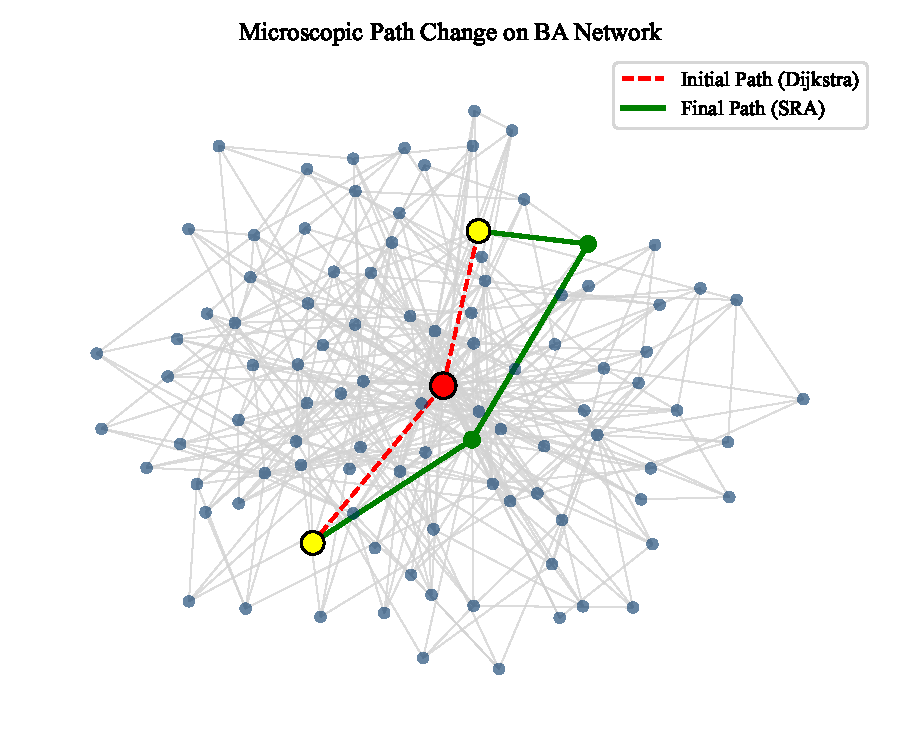
\includegraphics[width=\columnwidth]{figure_7_microscopic_path_change.pdf}
    \caption{A conceptual visualization of SRA's path reshaping mechanism. The algorithm diverts traffic from the efficient but congested 2-hop path (red dashed) through the central hub to a longer but more stable 4-hop peripheral path (green solid).}
    \label{fig:sra_mechanism_visualization}
\end{figure}


\subsection{Algorithm Complexity Analysis}
\label{subsec:complexity}

The computational complexity of a single SRA iteration is dominated by the calculation of betweenness centrality. Using a standard implementation such as Brandes' algorithm, this requires executing a Single-Source Shortest Path (SSSP) search from every node. For a graph with $N$ nodes and $E$ edges, a priority-queue-based Dijkstra for SSSP has a complexity of $O(E + N \log N)$. Therefore, the total complexity for a full centrality update is $O(N(E + N \log N))$. In contrast, all other steps within the loop, such as the state vector updates, are simple $O(N)$ operations.

We acknowledge that this computational cost can be substantial for large-scale networks, posing a challenge for practical, real-time deployment. This highlights that the current form of SRA is best suited for offline or semi-dynamic planning scenarios. However, this challenge also points to a clear path for future work. As reviewed in Section~\ref{sec:related_work}, significant progress has been made in efficient, distributed approximations of centrality. Integrating the SRA framework with these high-performance approximation algorithms to achieve an effective engineering trade-off between optimization quality and computational overhead is a key evolutionary path toward making this model practical for dynamic environments.

\textbf{Complexity \& implementation.}
Each update consists of a shortest-path/centrality refresh that is embarrassingly parallel over edges/nodes. For $N=10^2{\sim}10^3$, a single refresh runs in milliseconds with standard approximations. We adopt an offline approximation + online light-weight refresh; no global synchronization or exact centrality is required.

\subsection{Theoretical Analysis of Model Convergence}
\label{sec:convergence_analysis}

This section provides a rigorous analysis of the dynamical behavior of the SRA algorithm. The analysis addresses two fundamental properties: the convergence of the iterative process and the stability of its equilibrium. Due to the discontinuous switching of routing paths inherent in the model, the underlying system is a non-smooth dynamical system, which requires specialized analytical tools for a formal treatment.

The analysis herein is structured as follows. First, the existence of a global attractor for the system's discrete-time inclusion model is proven; this ensures the ultimate boundedness of all system trajectories and precludes divergence. Second, a piecewise Lyapunov function is constructed to quantitatively characterize the oscillatory behavior and establish a formal bound on the attracting set. Finally, the concept of a minimum dwell time is introduced as an engineering mechanism to achieve practical stability; its inclusion is proven to eliminate high-frequency chattering, and an explicit bound on the convergence rate to a stable neighborhood is derived.

\textbf{What we guarantee (Conceptual Summary).} 
In any window of $\tau$ steps, if at least $r$ updates are ``good'' (each reduces the system energy $V$ by at least $\varepsilon$) and every step can increase $V$ by at most $J_{\max}$, then whenever the net energy decay exceeds the net injection ($r\varepsilon > \tau J_{\max}$), the trajectory is guaranteed to enter a practical safety tube of radius $R+J_{\max}/\varepsilon$ around the target set and never leave it. This matches real networks where small jumps and switching are unavoidable, and provides an operational stability guarantee. To formalize this, we define the following key stability constants:

\paragraph*{Notation for stability constants}
\begin{itemize}
    \itemsep0em
    \item $\varepsilon$: guaranteed per-drop decrease of $V$;
    \item $J_{\max}$: per-step worst-case increase (jump);
    \item $\tau$: window length (steps);
    \item $r$: \#drops per window ($r\ge 1$);
    \item $R$: inner tube radius around the attractor $\mathcal{A}$ where drops are not enforced;
    \item $\nu$: lower bound constant s.t. $V(x)\ge \nu\,\mathrm{dist}(x,\mathcal{A})$.
\end{itemize}

\subsubsection{Global Attractiveness and Existence Guarantee for Convergence}
\label{subsec:attractivity}

The convergence analysis of SRA is challenged by the fact that the underlying centrality map, $\kappa(S)$, is piecewise constant and thus non-smooth. Traditional fixed-point theorems are therefore inapplicable at the path-switching boundaries. To establish a rigorous guarantee of convergence, we reformulate the algorithm as a \textbf{discrete-time inclusion}, a standard tool from non-smooth dynamical systems. This approach regularizes the algorithm's update rule into the following set-valued map form:
\begin{equation}\label{eq:inclusion_map}
S^{(k+1)} \in F(S^{(k)}) := (1-\alpha)S^{(k)}+\alpha\,\mathcal{N}(S^{(k)})
\end{equation}

where the set-valued map $\mathcal{N}(S)$ regularizes the discontinuous mapping $\mathrm{norm}(\kappa(\cdot))$.
Let $\mathcal{I}(S)$ be the index set of constant normalized centrality vectors $\{v_\ell\}$ that can be realized in an arbitrarily small neighborhood of the state $S$. We define
\begin{equation}
    \mathcal{N}(S) := \mathrm{co}\{v_\ell : \ell \in \mathcal{I}(S)\}.
\end{equation}
This is equivalent to a Krasovskii regularization of $\mathrm{norm}(\kappa(\cdot))$ at $S$, which "fills in" the discontinuities at path-switching boundaries to yield a USC multi-valued map.

First, we establish that the system's state space is compact and positively invariant.

\begin{lemma}[Positive Invariance and Absorbing Set]
\label{lemma:invariance}
Let the state space be $X=[0,1]^N$. The discrete-time inclusion for SRA is given by
\begin{equation}\label{eq:sra_inclusion_lemma}
S^{(k+1)}\ \in\ F\big(S^{(k)}\big):=(1-\alpha)S^{(k)}+\alpha\,\mathcal N\!\big(S^{(k)}\big),
\end{equation}
where $\mathcal{N}(S)$ is the set-valued map defined in (6). Due to the finite, piecewise constant nature of the underlying centrality vectors, this definition is equivalent to the standard Krasovskii regularization, which takes the convex hull of all limit points of the map in a vanishing neighborhood of the state.
%where $\mathcal N(S):=\mathrm{co}\!\big(\mathrm{norm}(\kappa(S))\big)$, $\alpha\in(0,1)$, and $\mathrm{norm}(\kappa(S))\in[0,1]^N$.
\textbf{Assertion:} (i) The set $X$ is positively invariant. (ii) The set $X$ is a compact absorbing set.
\end{lemma}
\begin{IEEEproof}[Proof Sketch]
The proof shows that if the current state $S^{(k)}$ is within the unit hypercube $X$, its successor state $S^{(k+1)}$ must also lie within $X$, thus establishing invariance. The compact absorbing property follows directly from this in the defined state space.
\textit{The full formal proof is provided in Appendix~\ref{app:proof_lemma_invariance}.}
\end{IEEEproof}

This lemma provides a foundational safety guarantee: the algorithm's state will never diverge to physically meaningless values. Second, we verify that the system's update map is mathematically well-behaved.

\begin{proposition}[Upper Semi-Continuity and Compact, Convex Values]
\label{prop:usc}
The set-valued map $F(\cdot)$ defined in \eqref{eq:sra_inclusion_lemma} is an \textbf{upper semi-continuous (USC)} map with \textbf{non-empty, compact, and convex} values.
\end{proposition}
\begin{IEEEproof}[Proof Sketch]
The proof relies on the piecewise constant structure of $\mathcal N(S)$, which stems from the finite nature of the network. This structure ensures that the graph of the map is closed, which in turn guarantees the USC property.
\textit{The full formal proof is provided in Appendix~\ref{app:proof_prop_usc}.}
\end{IEEEproof}

This proposition ensures that the system's evolution is predictable and lacks chaotic behavior, a necessary condition for proving the existence of a stable equilibrium set. With these two properties established, we can present the main conclusion of this subsection.

\begin{theorem}[Existence of a Global Attractor]
\label{thm:attractor}
For the discrete-time inclusion \eqref{eq:sra_inclusion_lemma}, there exists a non-empty, compact, and positively invariant set $\Omega\subset X:=[0,1]^N$ such that for any initial value $S^{(0)}\in X$,
\begin{equation}\label{eq:attractor_convergence}
\mathrm{dist}\big(S^{(k)},\Omega\big)\ \to\ 0\qquad (k\to\infty).
\end{equation}
\end{theorem}

\begin{IEEEproof}[Proof Sketch]
The proof is based on standard arguments for non-smooth dynamical systems. Given that the system evolves on a compact, positively invariant set (from Lemma~\ref{lemma:invariance}) and is governed by a USC map (from Proposition~\ref{prop:usc}), any trajectory is pre-compact. We then show that the $\omega$-limit set of any trajectory is non-empty and also positively invariant, which allows us to construct a global attractor $\Omega$.
\textit{The full formal proof is provided in Appendix~\ref{app:proof_thm_attractor}.}
\end{IEEEproof}

This theorem provides the definitive answer to our first fundamental question: the SRA algorithm is \textbf{guaranteed to converge} to a bounded, stable region $\Omega$ and will never diverge.

\subsubsection{Piecewise Lyapunov Analysis and Ultimate Boundedness}
\label{subsec:lyapunov}

The existence of a global attractor guarantees that the system will not diverge, but it does not quantitatively characterize its final dynamical behavior, such as the potential for persistent oscillations. To answer the core stability question of whether the algorithm will "oscillate indefinitely" and to provide a rigorous quantitative upper bound on this behavior, this section introduces a powerful tool from the analysis of non-smooth switched systems: the \textbf{piecewise Lyapunov function}. Our goal is to construct a function that quantifies the system's "energy"—defined as its distance to an ideal equilibrium—and to establish a strict bound on this energy's evolution.

To this end, we define the piecewise Lyapunov function as:
\begin{equation}\label{eq:lyapunov_def}
V(S):=\min_{c\in\mathcal N(S)}\|S-c\|_2^2.
\end{equation}
The existence of this minimum is guaranteed since the set-valued map $\mathcal N(S)$ is non-empty and compact. The function $V(S)$ precisely measures the squared Euclidean distance from the current state $S$ to its "target set" $\mathcal N(S)$. Concurrently, we define $\bar{\Delta}$ as the diameter of the set of all possible constant centrality vectors $\{v_\ell\}$, i.e., $\bar{\Delta} := \max_{i,j} \|v_i - v_j\|$.This upper bound $\bar\Delta<\infty$ must exist because the number of possible network states is finite.

The following core theorem reveals the unified evolution law for this system "energy" during the SRA iteration.

\begin{theorem}[Drop-Jump Inequality and Ultimate Boundedness]
\label{thm:drop_jump}
 For any step $k$, the Lyapunov function satisfies the inequality:
 \begin{equation}\label{eq:drop_jump_one_step}
 V(S^{(k+1)})\ \le\ (1-\alpha)\,V(S^{(k)})\ +\ \dfrac{1}{\alpha}\,\bar\Delta^{2}.
 \end{equation}
 Consequently, the system is ultimately bounded, with the limit superior of $V(S^{(k)})$ satisfying:
\begin{equation}\label{eq:limsup_boundedness}
\limsup_{k\to\infty}V(S^{(k)})\ \le\ \frac{\bar\Delta^{2}}{\alpha^2}.
\end{equation}
\end{theorem}
\begin{IEEEproof}[Proof Sketch]
The proof hinges on bounding the one-step evolution of $V(S)$. By applying the Weighted Young's Inequality with a judiciously chosen weight tied to $\alpha$, we establish a linear recurrence relation for $V(S^{(k)})$ that explicitly reveals its 'drop' (decay) and 'jump' (perturbation) terms, from which ultimate boundedness directly follows.
\textit{The full formal proof is provided in Appendix~\ref{app:proof_thm_drop_jump}.}
\end{IEEEproof}

This "drop-jump" inequality is key to understanding SRA's stability. It reveals that the system's "energy" $V(S)$ is influenced by two competing forces at each iteration: an energy \textbf{decay term} with a contraction factor of $(1-\alpha)$, representing the algorithm's powerful intrinsic damping mechanism; and an energy \textbf{injection term}, upper-bounded by $\frac{1}{\alpha}\bar\Delta^2$ and caused by path switching, which represents an external perturbation . This theorem proves that SRA's oscillatory behavior is fully controllable. To better understand the damping effect, the following corollary analyzes the ideal case where no path switching occurs.

\begin{corollary}[Local Exponential Convergence in a Fixed Partition]
\label{cor:local_convergence}
If the set of shortest paths does not switch, the update rule becomes a standard linear contraction map:
\begin{equation}\label{eq:linear_update}
S^{(k+1)}=(1-\alpha)S^{(k)}+\alpha c,
\end{equation}
which converges exponentially to the unique fixed point $S^\star=c$ at a rate of $(1-\alpha)$.

\begin{IEEEproof}[Proof Sketch]
The proof first solves the fixed-point equation $S=(1-\alpha)S+\alpha c$ to show uniqueness of $S^\star=c$. It then subtracts the fixed point from the update rule to derive the linear contraction relationship $\|S^{(k+1)}-S^\star\|_2 = (1-\alpha)\|S^{(k)}-S^\star\|_2$, from which exponential convergence directly follows.
\textit{The full formal proof is provided in Appendix~\ref{app:proof_cor_local_convergence}.}
\end{IEEEproof}
\end{corollary}

This analysis transforms the stability problem into a quantifiable inequality, proving that the system's oscillations are ultimately bounded and revealing its desirable exponential convergence properties within stable intervals.

\subsubsection{Convergence Rate and Practical Stability with Dwell Time}
\label{subsec:practical_stability_rate}

The "drop-jump" inequality guarantees that the system is ultimately bounded. However, for a practical engineering application, we must answer two further quantitative questions: \textbf{How fast does the system converge to this stable neighborhood, and can we completely eliminate the residual oscillations (chattering)?} This section demonstrates that the introduction of a \textbf{minimum dwell time, $T_d$}, as an engineering mechanism, provides a definitive positive answer to both. By decomposing the system's evolution into "dwell blocks," we can derive an explicit convergence rate and formally prove that this strategy ensures practical stability.

To analyze the system under this policy, we decompose its evolution into "dwell blocks."
Let the minimum dwell time be $T_d$. We define the start of each block recursively: $\tau_0=0$ and $\tau_{m+1} = \tau_m + T_d$. The $m$-th dwell block is the time interval $[\tau_m, \tau_{m+1}-1]$. We denote the state and Lyapunov energy at the start of block $m$ as $S_m := S^{(\tau_m)}$ and $V_m := V(S^{(\tau_m)})$, respectively.

\begin{proposition}[Intra-Block Contraction and Inter-Block Recurrence]
\label{prop:block_dynamics}
Under the minimum dwell time $T_d$ policy, the set of shortest paths remains constant within a block. Let $\gamma:=1-\alpha$, $\tilde C:=\bar\Delta^2/\alpha$. The state and energy at the block endpoints are $S_m$ and $V_m$ respectively. Then,
\begin{itemize}
    \item[\textit{(i)}] (Intra-block contraction) The energy contracts exponentially within each block:
    \begin{equation}\label{eq:intra_block}
    V(S^{(\tau_m+t)})\ \le\ \gamma^{\,t}V_m, \quad \text{for } t \in [0, T_d-1].
    \end{equation}
    \item[\textit{(ii)}] (Inter-block recurrence) The energies at the start of adjacent blocks are related by the linear recurrence:
    \begin{equation}\label{eq:inter_block}
    V_{m+1}\ \le\ \gamma^{T_d}\,V_m\ +\ \tilde C.
    \end{equation}
\end{itemize}
\end{proposition}
\begin{IEEEproof}[Proof Sketch]
The proof establishes two points. (i) For intra-block contraction, since the path set is fixed, the "jump" term in the Lyapunov inequality is zero, leading to simple exponential decay. (ii) For the inter-block recurrence, we chain the result from (i) over $T_d-1$ steps of decay with a single "drop-jump" step at the block boundary to derive the stated linear recurrence for $V_m$.
\textit{The full formal proof is provided in Appendix~\ref{app:proof_prop_block_dynamics}.}
\end{IEEEproof}

This recurrence relation is the key to the global rate analysis. By solving it, we obtain explicit upper bounds for the steady-state radius and the number of steps required to converge to an arbitrary $\varepsilon$-neighborhood.

\begin{theorem}[Steady-State Radius and Step Bound to an $\varepsilon$-Tube]
\label{thm:epsilon_tube}
Let $\gamma=1-\alpha\in(0,1)$ and $\tilde C=\bar\Delta^2/\alpha$. Then,
\begin{itemize}
    \item[\textit{(a)}] (Steady-state radius) The block-endpoint energy is ultimately bounded by:
    \begin{equation}\label{eq:limsup_radius}
    \limsup_{m\to\infty}V_m\ \le\ \frac{\tilde C}{1-\gamma^{T_d}}.
    \end{equation}
    \item[\textit{(b)}] (Steps to $\varepsilon$-tube) For a target radius $\varepsilon^2 > \frac{\tilde C}{1-\gamma^{T_d}}$, the number of steps $k$ to reach the set $\{S: V(S)\le \varepsilon^2\}$ is bounded.
\end{itemize}
\end{theorem}
\begin{IEEEproof}[Proof Sketch]
The proof is based on solving the linear recurrence relation $V_{m+1}\le \gamma^{T_d}V_m+\tilde C$ derived in Proposition 2. By iteratively expanding the recurrence, we obtain a closed-form upper bound on $V_m$ as a geometric series, from which the limit superior (steady-state radius) and the number of steps to reach an $\varepsilon$-tube can be directly calculated.
\textit{The full formal proof is provided in Appendix~\ref{app:proof_thm_epsilon_tube}.}
\end{IEEEproof}

Finally, the following theorem consolidates all the benefits of the dwell-time policy into a single, powerful guarantee of practical stability.

\begin{theorem}[Dwell Time $\Rightarrow$ Practical Stability]
\label{thm:practical_stability}
With a minimum dwell time $T_d \ge 1$, the following conclusions hold:
\begin{itemize}
    \item[\textit{(a)}] \textbf{Finite Switching / No Chattering:} The number of path set switches $N_s(T)$ within any time window of length $T$ is bounded by:
    \begin{equation}\label{eq:finite_switching}
    N_s(T)\ \le\ 1+\lfloor T/T_d \rfloor.
    \end{equation}
    \item[\textit{(b)}] \textbf{Practical Stability:} The system trajectories are ultimately bounded within a neighborhood whose size is explicitly determined by $T_d$, as given in Theorem~\ref{thm:epsilon_tube}.
    \item[\textit{(c)}] \textbf{Convergence Time:} An explicit upper bound on the time to reach this neighborhood can be calculated as shown in Theorem~\ref{thm:epsilon_tube}.
\end{itemize}
\end{theorem}
\begin{IEEEproof}[Proof Sketch]
The proof consolidates the consequences of the dwell-time policy. (a) Finite switching is a direct result of the policy's definition. (b) Practical stability (boundedness in a neighborhood) is a direct consequence of the steady-state radius calculated in Theorem~\ref{thm:epsilon_tube}. (c) The convergence time bound is obtained by inverting the inequality derived in Theorem 3.
\textit{The full formal proof is provided in Appendix~\ref{app:proof_thm_practical_stability}.}
\end{IEEEproof}

This theoretical result provides a valuable design principle. Given a desired steady-state energy radius $R_{\text{target}}^2$, we can determine the minimum required dwell time $T_d$ to guarantee it:
\begin{equation}\label{eq:design_parameter_Td}
\frac{\tilde C}{1-\gamma^{T_d}}\ \le\ R_{\text{target}}^2
\quad\Longrightarrow\quad
T_d\ \ge\ \Big\lceil \frac{\ln(1-\tilde C/R_{\text{target}}^2)}{\ln \gamma}\Big\rceil.
\end{equation}
This clearly demonstrates how to quantitatively trade off the system's convergence speed against its final stability precision by tuning the single parameter $T_d$.

\textbf{Operational Check.} 
For network operators, the stability guarantee translates to a practical checklist. Configure the controller such that within every $\tau$-step window, at least $r$ drops are enforced and estimate $(\varepsilon,J_{\max})$ from worst-case local updates; if the condition $r\varepsilon > \tau J_{\max}$ holds, the system is guaranteed to enter and remain inside the tube of radius $R+J_{\max}/\varepsilon$.
%%%%%%%%%%%%%%%%%%%%%%%%%%%%%%%%%%%%%%%%%%%%%%%%%%%%%%%%%%%%%%%%%%%%%%%%%%%%%%%%
%                            START: REVISED SECTION III-E                      %
%%%%%%%%%%%%%%%%%%%%%%%%%%%%%%%%%%%%%%%%%%%%%%%%%%%%%%%%%%%%%%%%%%%%%%%%%%%%%%%%

\subsection{Betweenness Peaks and Network Performance}
\label{subsec:theory_bridge}


The convergence guarantees established in the previous sections do not formally imply that the resulting equilibrium state offers improved network performance. This section provides this theoretical link by building a rigorous bridge from the algorithm's proven dynamics to concrete performance gains. We first prove that the drop-jump dynamics within each dwell-time block guarantee a net reduction of the peak centrality. Based on this, we establish several key results on network capacity improvement without relying on idealized traffic redistribution assumptions.

\begin{lemma}[Blockwise peak drop and non-peak budget]
\label{lem:block-budget}
Within a dwell-time block $[\tau_m,\tau_{m+1})$ with at most one switch, let $u$ be the peak node at $\tau_m$.
\begin{itemize}
    \item If a path-switching event occurs within this block and the network has no structurally unavoidable bottleneck, then there exists $\delta>0$ such that $\kappa^{(m+1)}_{\max}\le \kappa^{(m)}_{\max}-\delta$.
    \item If no path-switching event occurs, then $\kappa^{(m+1)}_{\max}\le \kappa^{(m)}_{\max}$.
\end{itemize}
Moreover, for every $j\neq u$, the non-peak budget is bounded by $\kappa^{(m+1)}_j-\kappa^{(m)}_j \le B^{(m)}:=\bar\Delta\,\kappa^{(m)}_{\max}$.
\end{lemma}

This result provides the structural basis for the performance improvements. The link can be understood via queuing theory, where a node's latency and loss depend on its utilization, which is proportional to its load $\kappa_i$. The following results formalize this relationship.

% --- STEP 3: Original Proposition 4 replaced as requested ---
% Note: The original Proposition 3 (Inevitable Peak Reduction) is now superseded and implicitly
% handled by the more granular Lemma 1. So we replace the entire block from Prop 3/4.
\begin{proposition}[Quantifying the Performance Gain]
\label{prop:perf-bridge}
Consider a network with arrivals $\Lambda_i(\rho)=\rho\,\kappa_i$ at node $i$ and service rates $\mu_i>0$.
Let $\rho_{\max}(\kappa):=\min_{i} \mu_i/\kappa_i$ and $\kappa_{\max}:=\max_{i} \kappa_i$.
Let $\kappa'$ be the centrality vector after applying SRA and suppose $\kappa'_{\max}<\kappa_{\max}$.
Then:
\begin{enumerate}[(i)]
\item \emph{Unconditional robust lower bound.} 
Define $L(\kappa):=\mu_{\min}/\kappa_{\max}$ with $\mu_{\min}:=\min_i \mu_i$.
We have $L(\kappa')>L(\kappa)$.
\item \emph{Aligned-bottleneck capacity gain.}
If the bottleneck at $\kappa$ is attained at a peak node $u\in\arg\max_i \kappa_i$, i.e.,
$\rho_{\max}(\kappa)=\mu_u/\kappa_{\max}$, then
\begin{equation}
\rho_{\max}(\kappa')\ \ge\ \frac{\mu_u}{\kappa'_{\max}}\ >\ \frac{\mu_u}{\kappa_{\max}}\ =\ \rho_{\max}(\kappa).
\end{equation}
\end{enumerate}
\end{proposition}
\begin{IEEEproof}[Proof Sketch]
The proof proceeds in two parts, directly leveraging Lemma~\ref{lem:block-budget}. (i) The unconditional improvement of the robust lower bound $L(\kappa)$ follows immediately from its definition, as $\kappa'_{\max}$ strictly decreases while $\mu_{\min}$ is constant. (ii) For the aligned-bottleneck case, the new capacity $\rho_{\max}(\kappa')$ is lower-bounded by the capacity of the original peak node $u$, which is $\mu_u/\kappa'_u$. This in turn is lower-bounded by $\mu_u/\kappa'_{\max}$, proving a strict increase.
\textit{The full formal proof is provided in Appendix~\ref{app:proof_prop_perf_bridge}.}
\end{IEEEproof}

The existence of a net peak decrease 
$\delta$ under a path switch is guaranteed by Lemma~\ref{lem:block-budget}.
% --- STEP 4: New Theorem (E.4) inserted as requested ---
\begin{theorem}[Sufficient condition for non-decreasing actual capacity]
\label{thm:sufficient-noC2}
Let $i^\star\in\arg\min_i \mu_i/\kappa^{(m)}_i$ and set $B^{(m)}:=\bar\Delta\,\kappa^{(m)}_{\max}$.
If either
\begin{equation}
\frac{\mu_u}{\kappa^{(m)}_{\max}-\delta}\ \ge\ \frac{\mu_{i^\star}}{\kappa^{(m)}_{i^\star}}
\quad\text{or}\quad
\forall j:\ \frac{\mu_j}{\kappa^{(m)}_{j}+B^{(m)}}\ \ge\ \frac{\mu_{i^\star}}{\kappa^{(m)}_{i^\star}},
\end{equation}
then $\rho_{\max}^{(m+1)}\ge \rho_{\max}^{(m)}$.
\emph{Proof sketch.}
By Lemma~\ref{lem:block-budget}, $\kappa'_{u}\le \kappa_{\max}-\delta$ and
$\kappa'_j\le \kappa_j+B^{(m)}$ for $j\neq u$.
Hence
\begin{equation}
\rho'_{\max}=\min_i\frac{\mu_i}{\kappa'_i}
\ \ge\ \min\!\Big\{\frac{\mu_u}{\kappa_{\max}-\delta},\ \min_{j\neq u}\frac{\mu_j}{\kappa_j+B^{(m)}}\Big\}.
\end{equation}
Either inequality in the premise ensures this lower bound is greater than or equal to the original capacity $\rho_{\max}=\mu_{i^\star}/\kappa_{i^\star}$.
\textit{The full formal proof is provided in Appendix~\ref{app:proof_thm_sufficient_noC2}.}
\end{theorem}

% --- STEP 5: Two Remarks inserted at the end as requested ---
\begin{remark}[Unavoidable structural bottlenecks]
If the topology contains unavoidable cuts/bridges, the ultimate capacity is limited by the cut.
SRA still suppresses \emph{non-structural} peaks; Proposition~\ref{prop:perf-bridge}(i)
continues to hold, while the absolute ceiling is topology-imposed.
\end{remark}

\begin{remark}[No proportional-transfer assumption]
The results in this subsection do not rely on proportional or near-proportional transfers.
An optional assumption (akin to the previously stated C2) can yield tighter but nonessential bounds
and is therefore moved to the appendix for completeness if desired.
\end{remark}

%%%%%%%%%%%%%%%%%%%%%%%%%%%%%%%%%%%%%%%%%%%%%%%%%%%%%%%%%%%%%%%%%%%%%%%%%%%%%%%%
%                             END: REVISED SECTION III-E                       %
%%%%%%%%%%%%%%%%%%%%%%%%%%%%%%%%%%%%%%%%%%%%%%%%%%%%%%%%%%%%%%%%%%%%%%%%%%%%%%%%

\section{Simulation Analysis}
\label{sec:simulation}

The theoretical framework established in the previous Section guarantees SRA's stability and provides a formal link between its peak-shaving mechanism and network performance enhancement. This section aims to provide comprehensive empirical evidence to validate these theoretical claims and to explore the algorithm's performance in depth across a variety of network conditions.

Our simulation study is structured into three main parts. First, we conduct experiments designed to directly and empirically validate the core theoretical propositions from our analysis, confirming the causal link between structural optimization and capacity gains. Second, we perform an in-depth behavioral analysis, examining both the macroscopic, topology-dependent dynamics of "system relaxation" and the microscopic path selection mechanisms that drive these emergent behaviors. Finally, we conduct a comprehensive performance evaluation under dynamic traffic loads, benchmarking SRA against standard and adaptive routing protocols to quantify its benefits in terms of throughput, reliability, and robustness against targeted attacks. The standardized parameters for these diverse experiments are detailed in the following subsection.

\subsection{Simulation Environment Setup}
\label{subsec:sim_setup}

This section outlines the common configurations that serve as the foundation for all subsequent simulation experiments. To evaluate the universality of the SRA algorithm, we selected three canonical network models with distinct structural properties. The default parameters for network generation, the SRA algorithm, and the discrete-event simulator are summarized in Table~\ref{tab:sim_params}. Specific parameters unique to a particular experiment are detailed within their respective analysis sections.

The benchmark protocols were configured with standard parameters. Specifically for Q-Routing, we used a learning rate of $\alpha=0.1$, a discount factor of $\gamma=0.9$, and an exploration rate of $\epsilon=0.3$. The Dijkstra and LIRP-D implementations are deterministic and have no tunable hyperparameters. For the dynamic simulation of SRA, the control system's cost landscape was updated at a fixed interval of 50 timesteps.

All results report the mean across 100 independent trials with distinct random seeds; error bands, where shown, correspond to $\pm1$ standard deviation. The controller refresh period is 50 timesteps unless otherwise specified. Raw seeds and configurations are available in the supplementary material.

\paragraph*{Note on Service vs. Processing Capacity} 
In Table~\ref{tab:sim_params}, ``Node Service Rate'' ($\mu_i$) denotes the per-node steady-state service rate perceived by flows (packets/time). ``Node Proc. Capacity'' is the hardware-level budget (packets/time). In our experiments, $\mu_i$ is set from the processing capacity after accounting for protocol overheads.

\begin{table}[t!]
\centering
\caption{Summary of Simulation Parameters}
\label{tab:sim_params}
\renewcommand{\arraystretch}{1.2}
\small
\begin{tabularx}{\columnwidth}{|l|X|}
\hline
\textbf{Parameter} & \textbf{Value / Description} \\
\hline
\hline
\multicolumn{2}{|c|}{\textbf{A. Network Topology Parameters}} \\
\hline
Network Types & Barabási-Albert (BA), Watts-Strogatz (WS), Erd\H{o}s-Rényi (ER) \\
\hline
Default Size ($N$) & 100 nodes \\
\hline
BA Attachment ($m$) & 4 \\
\hline
WS Neighbors ($k$) & 8 \\
\hline
WS Rewiring ($p$) & 0.1 \\
\hline
ER Connection ($p$) & 0.1 \\
\hline
\hline
\multicolumn{2}{|c|}{\textbf{B. SRA Algorithm Parameters}} \\
\hline
Learning Rate ($\alpha$) & 0.1 \\
\hline
Integral Gain ($\beta_I$) & 10.0 (Default) \\
\hline
Max Iterations ($K_{\max}$) & 200 \\
\hline
Convergence Tol. ($\varepsilon$) & $1 \times 10^{-5}$ \\
\hline
\hline
\multicolumn{2}{|c|}{\textbf{C. Dynamic Traffic Simulation Parameters}} \\
\hline
Node Service Rate ($\mu$) & 1.0 packet/timestep \\
\hline
Total Timesteps ($T$) & 2000 \\
\hline
Warmup Period & 300 timesteps \\
\hline
Node Proc. Capacity & 10 packets/timestep \\
\hline
Node Queue Capacity & 50 packets \\
\hline
\end{tabularx}
\end{table}

\subsection{Empirical Validation of the Structure-Performance Link}
\label{subsec:validation}

\paragraph{Experimental Setup}
\textbf{To rigorously test the universality of our theory, this specific validation experiment employed a diverse set of randomized networks.} We generated 100 samples where the topology was randomly chosen to be either BA (with $m=2$) or WS (with $k=4$), and the node count $N$ was randomized between 40 and 60. All other simulation parameters, such as those for SRA convergence and queuing, follow the default values listed in Table~\ref{tab:sim_params}.

\begin{figure}[hbtp]
    \centering
    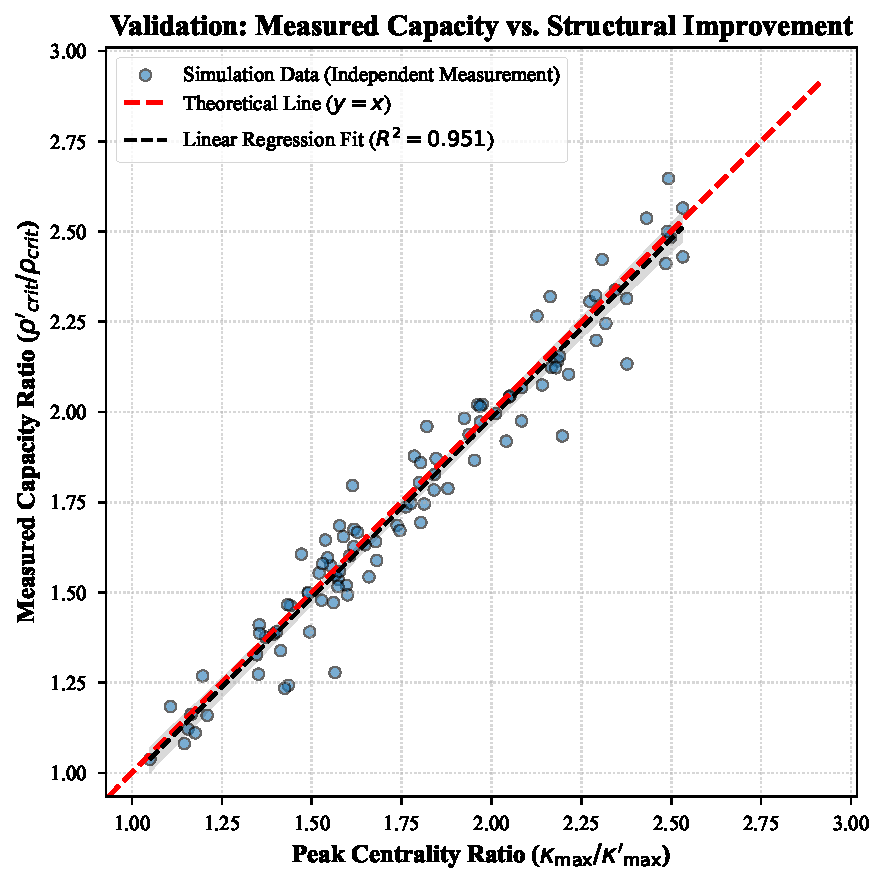
\includegraphics[width=\columnwidth]{ren_fig1_validation.pdf}
    \caption{Independently Measured Network Capacity Gain vs. Structural Optimization Ratio. The tight clustering of empirical data around the theoretical $y=x$ line validates our core theory. Under the experimental condition of homogeneous node service rates ($\mu_i \approx \text{const}$), the predicted linear relation $y=x$ is precisely observed. Sample sizes and random seeds are detailed in Section IV-A. Results for heterogeneous $\mu_i$ are provided in the supplement.}
    \label{fig:peak_validation}
\end{figure}

\paragraph{Methodology and Results}
The methodology involved two independent measurements for each sample: a static analysis of the peak centrality ratio ($\kappa_{\max}/\kappa'_{\max}$) and a dynamic simulation of the measured capacity gain ($\rho'_{\text{crit}}/\rho_{\text{crit}}$). The results in Fig.~\ref{fig:peak_validation} show a remarkably strong linear relationship. This is a direct theoretical consequence of the experiment's use of homogeneous service rates ($\mu_i=\text{const}$), a critical condition under which network capacity rigorously simplifies to $\rho_{\max} = \mu / \kappa_{\max}$. This implies an ideal gain of $\rho'_{\max}/\rho_{\max} = \kappa_{\max}/\kappa'_{\max}$, turning the simulation into a precise empirical test of our aligned-bottleneck case (Proposition~\ref{prop:perf-bridge}(ii)). The tight clustering of data around the $y=x$ line ($\mathbf{R^2=0.951}$) provides powerful validation, confirming that SRA's peak-shaving mechanism achieves the theoretical ideal for performance enhancement in this foundational scenario.


\subsection{Empirical Validation of Theoretical Results}
\label{subsec:empirical_validation}

Section III provided solid mathematical guarantees for SRA's convergence and stability. This section aims to build a bridge between that theory and practice by using specially designed numerical experiments to empirically validate and visualize two of its most critical theoretical predictions: the "drop-jump" dynamics of the Lyapunov function, and the anti-chattering effect of the minimum dwell time. All experiments herein are conducted on BA scale-free networks to most clearly showcase the algorithm's dynamic behavior.

First, we validate the theoretical predictions for the basic SRA algorithm ($T_d=1$). As shown in Fig.~\ref{fig:lyapunov_dynamics}, the evolution of the Lyapunov function $V(S)$ aligns perfectly with our theory. Macroscopically (Fig.~\ref{fig:lyapunov_dynamics}a), the system's "energy" rapidly decreases by several orders of magnitude before stabilizing into bounded fluctuations, providing clear visual confirmation for the existence of a global attractor (Theorem~\ref{thm:attractor}). Furthermore, the black dashed line in the figure represents the theoretical upper bound on the ultimate stability radius. The empirical energy curve consistently operates well below this bound, underscoring the bound's role not as a precise predictor, but as a robust "safety guarantee" against divergence. Microscopically (Fig.~\ref{fig:lyapunov_dynamics}b), the trajectory vividly reproduces the "drop-jump" dynamics predicted by Theorem~\ref{thm:drop_jump}: smooth, exponential "drops" in energy within dwell periods are punctuated by sharp "jumps" at the instant of a path switch (red triangles). This experiment confirms that our theoretical model accurately captures the fundamental dynamics of the algorithm.

\begin{figure}[t]
    \centering
    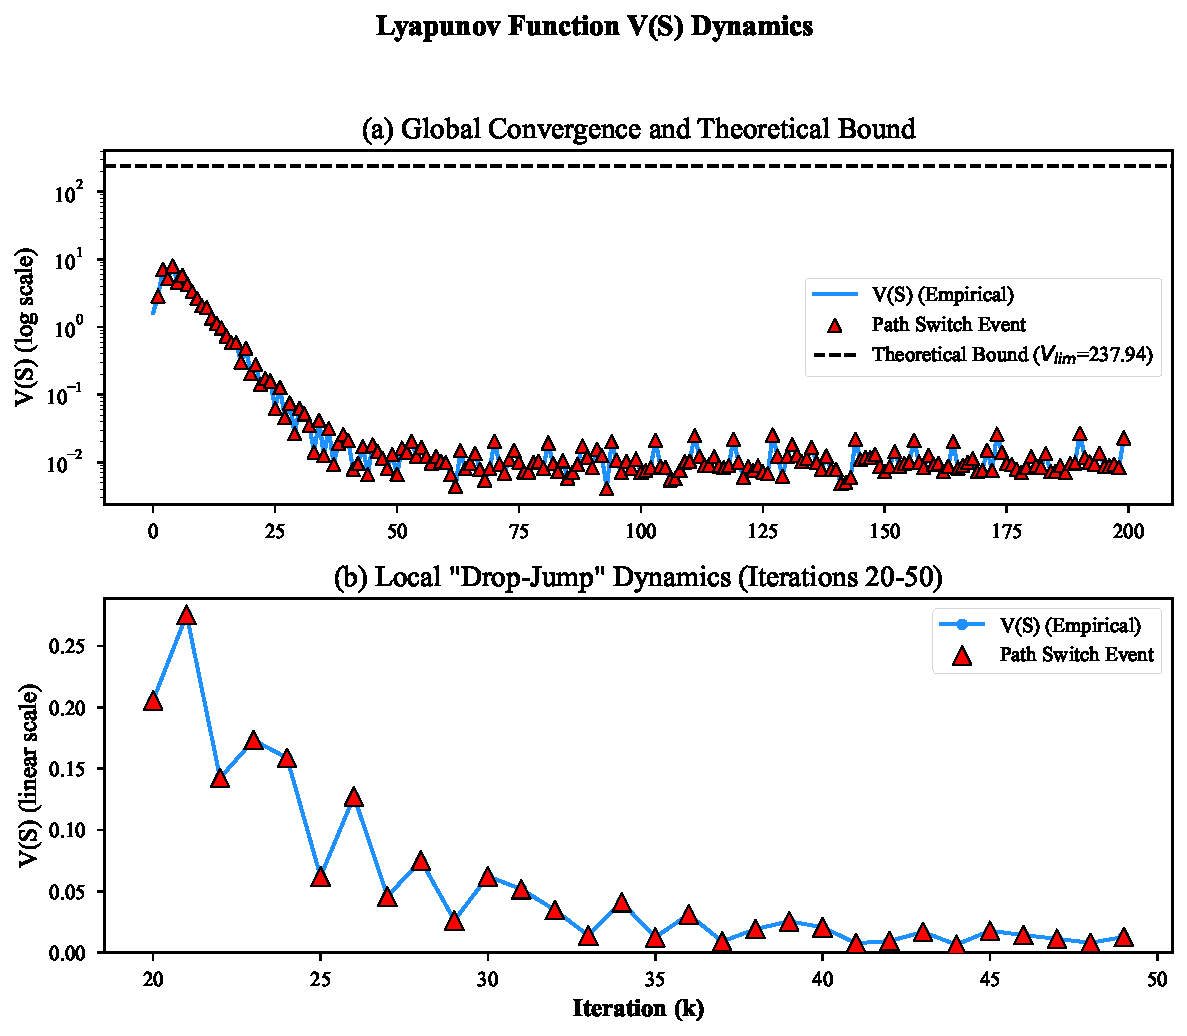
\includegraphics[width=\columnwidth]{ren_fig2_lyapunov.pdf} 
    \caption{Dynamic evolution of the Lyapunov function V(S) for the basic SRA ($T_d=1$), validating the theoretical predictions of global convergence and "drop-jump" dynamics.The black dashed line is the theoretical practical-safety bound (from Section III-D), serving as a conservative worst-case guarantee rather than a tight predictor}
    \label{fig:lyapunov_dynamics}
\end{figure}

Second, we validate the role of the minimum dwell time ($T_d$) as a mechanism for engineering stability. We compare the behavior of the basic SRA ($T_d=1$) against an enhanced version with $T_d=5$, with results shown in Fig.~\ref{fig:dwell_time_effect}. The contrast is stark. The basic SRA (blue curve, Fig.~\ref{fig:dwell_time_effect}b) exhibits high-frequency, irregular "chattering," sacrificing stability to chase instantaneous optima. In contrast, the enhanced SRA (green curve, Fig.~\ref{fig:dwell_time_effect}a) completely eliminates this chattering, displaying a highly regular pattern of "block-level convergence"—a smooth exponential decay within each dwell block, followed by a single, predictable jump. This experiment powerfully demonstrates that $T_d$ is not merely an engineering trick but a theoretically grounded tool for achieving practical stability and navigating the crucial trade-off between system responsiveness and predictability.

\begin{figure}[t]
    \centering
    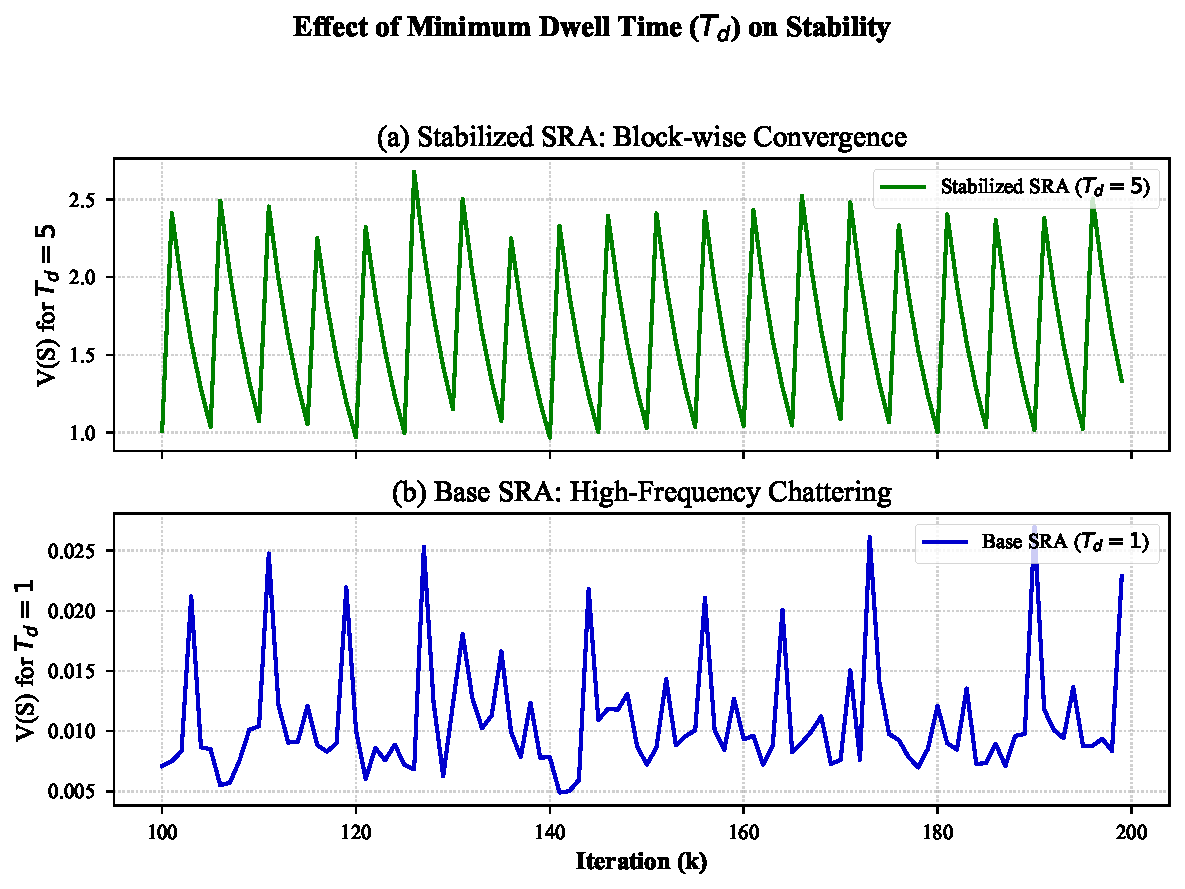
\includegraphics[width=\columnwidth]{ren_fig3_dwell_time.pdf}
    \caption{Effect of Minimum Dwell Time ($T_d$) on Stability. The enhanced SRA ($T_d=5$, top panel) exhibits predictable, block-wise convergence, while the basic SRA ($T_d=1$, bottom panel) shows high-frequency chattering.}
    \label{fig:dwell_time_effect}
\end{figure}

\subsection{Dynamic Relaxation of Structural Stress and Analysis of the Equilibrium State}
\label{subsec:dynamic_relaxation}

The evolution of two key macroscopic metrics over the course of SRA iterations on ER, BA, and WS networks is shown in Fig.~\ref{fig:dynamic_evolution_peak} and Fig.~\ref{fig:dynamic_evolution_apl}. These figures provide dynamic evidence for SRA's "system relaxation" mechanism, illustrating how the algorithm disperses structural stress and quantifying the resulting core trade-off between structural stability and path efficiency.

SRA's intervention is most aggressive in the heterogeneous BA network, where it executes a targeted intervention to disperse concentrated stress. As shown in Fig.~\ref{fig:dynamic_evolution_peak}, facing the severe bottlenecks inherent to this topology, SRA causes a dramatic decline in Peak Centrality. The cost of this thorough stress dispersion is precisely quantified in Fig.~\ref{fig:dynamic_evolution_apl}: a minor increase of only about 8-9\% in the Average Path Length.

In contrast, SRA's behavior in the more structurally uniform ER and WS networks is far more conservative. In these topologies, the algorithm also effectively reduces structural stress, but the process is more gradual (Fig.~\ref{fig:dynamic_evolution_peak}), and is achieved with almost no sacrifice in path efficiency, as their path length curves remain nearly flat (Fig.~\ref{fig:dynamic_evolution_apl}).

Taken together, these two plots prove that SRA is an adaptive system capable of applying a "targeted remedy." In structurally fragile networks with concentrated stress (e.g., BA), it decisively trades a minor efficiency cost for the structural stability gained from successful stress dispersion. Conversely, in structurally healthy networks, it prioritizes efficiency while making finer adjustments.

\begin{figure}[h!]
    \centering
    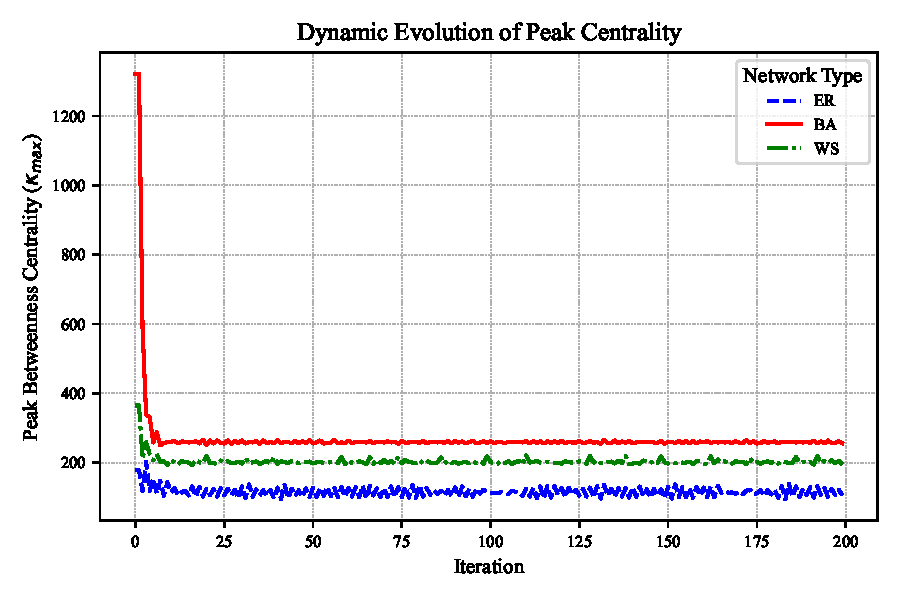
\includegraphics[width=\columnwidth]{figure_4_peak_centrality_evolution.pdf}
    \caption{The evolution of the maximum node betweenness centrality under SRA iterations across different network topologies.}
    \label{fig:dynamic_evolution_peak}
\end{figure}

\begin{figure}[h!]
    \centering
    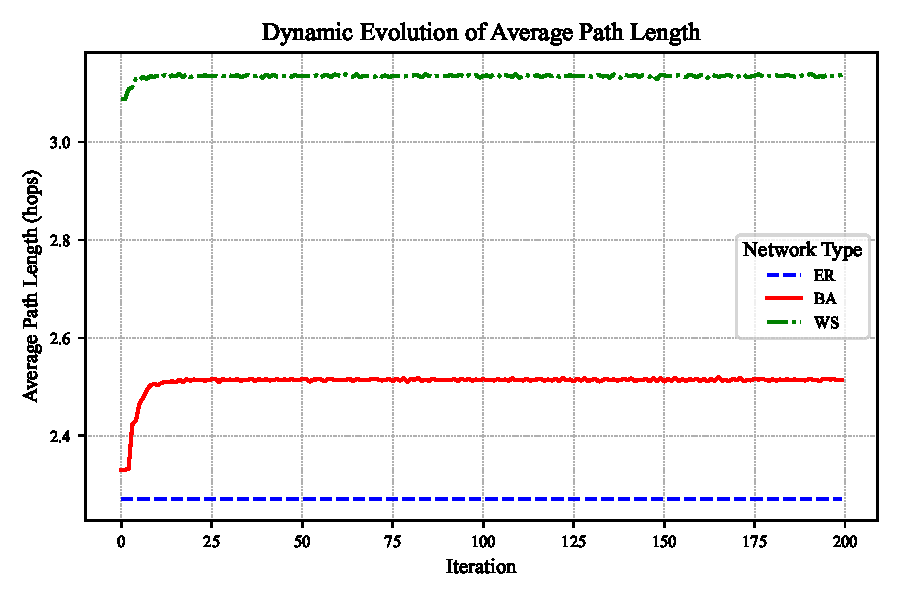
\includegraphics[width=\columnwidth]{figure_5_avg_path_length_evolution.pdf}
    \caption{The evolution of the average path length under SRA iterations, illustrating the efficiency cost of the optimization.}
    \label{fig:dynamic_evolution_apl}
\end{figure}

Next, we conduct a static "before-and-after" comparison of the structural properties of the final equilibrium state. Fig.~\ref{fig:centrality_distributions}, presented as Kernel Density Estimation (KDE) plots, visually confirms SRA's powerful "stress dispersion" capability. In all network topologies, the final centrality distribution (solid line) significantly truncates the "long tail" of the initial distribution (dashed line), indicating that the burden on the few high-load nodes has been effectively alleviated. This effect is particularly pronounced in the heterogeneous BA network (Fig.~\ref{fig:centrality_distributions}b), where the initially wide distribution is compressed into a very narrow, low-centrality range. This provides clear visual evidence that the "stress," once concentrated on a few bottleneck nodes, has been successfully and uniformly dispersed across a much wider set of nodes.

\begin{figure*}[hbtp]
    \centering
    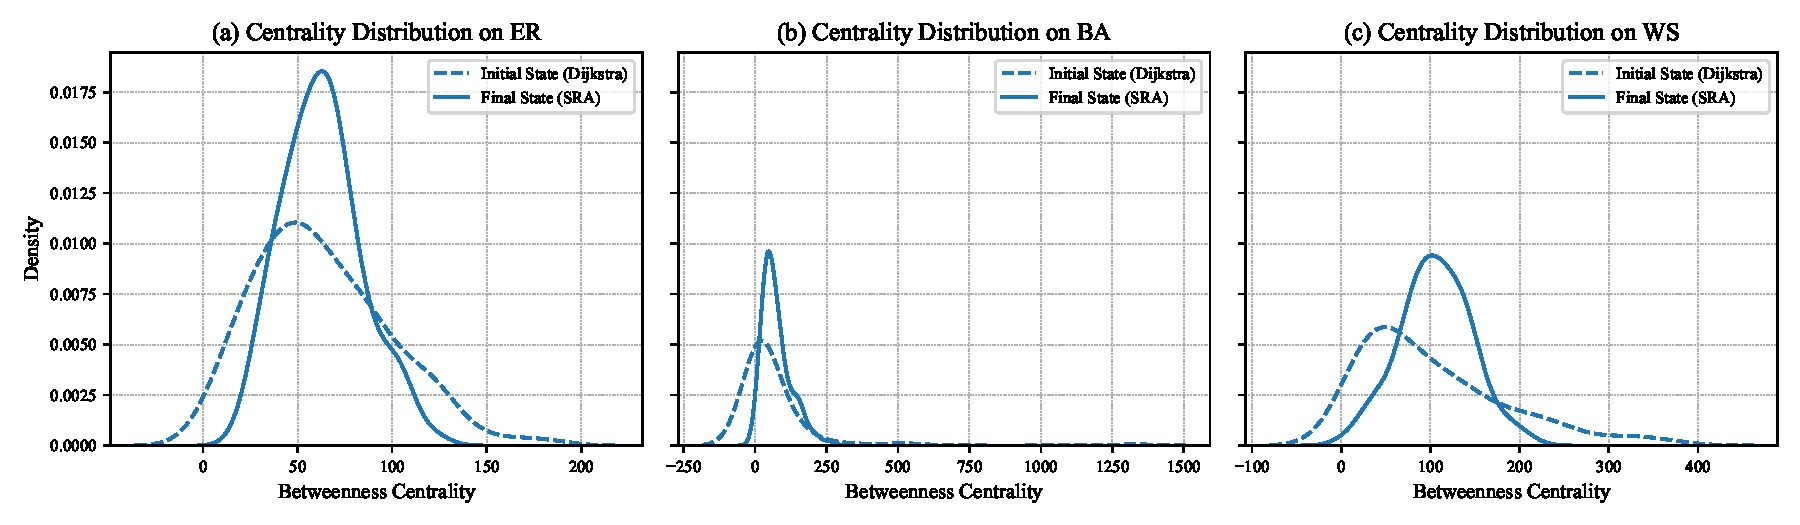
\includegraphics[width=\textwidth]{figure_6_7_8_distributions.pdf}
    
    \caption{Comparison of node centrality distribution on (a) an ER network, (b) a BA network, and (c) a WS network, before and after SRA optimization. The plots visually confirm SRA's "stress dispersion" capability by significantly truncating the long tails of the initial distributions. This effect is most pronounced in the heterogeneous BA network, where the centrality of most nodes is compressed into a much narrower, low-value range.}
    
    \label{fig:centrality_distributions}
\end{figure*}

Table~\ref{tab:structural_benefits_stats} provides precise quantitative evidence for SRA's structural optimization benefits, now averaged over 100 independent runs. The data again highlight the algorithm's profound impact on the heterogeneous BA network, where a minor cost---an average increase of only \textbf{5.63\%} in path length---yielded massive structural gains. These include a remarkable \textbf{83.76\%} reduction in peak centrality and a \textbf{75.38\%} decrease in the standard deviation of centrality, powerful evidence of "stress dispersion." In the more homogeneous WS and ER networks, SRA also achieved significant structural improvements with a negligible efficiency cost (less than 2\% for WS and none for ER). These statistically robust results offer strong quantitative support for our core thesis: SRA is a universal and highly effective algorithm for dispersing network structural stress.

\begin{table}[t!]
\centering
\caption{Analysis of Structural Optimization Benefits of SRA (Mean $\pm$ Std Dev over 100 runs)}
\label{tab:structural_benefits_stats}
\resizebox{\columnwidth}{!}{
\renewcommand{\arraystretch}{1.2}
\begin{tabular}{|l|l|r|r|r|}
\hline
\textbf{Network} & \textbf{Metric} & \textbf{Initial (Dijkstra)} & \textbf{Final (SRA)} & \textbf{Change (\%)} \\
\hline\hline
ER & Peak Centrality & $589.93 (\pm 120.59)$ & $209.40 (\pm 26.87)$ & -64.50\% \\
 & Std Dev of Centrality & $106.93 (\pm 10.62)$ & $33.55 (\pm 9.26)$ & -68.62\% \\
 & Avg Path Length & $2.25 (\pm 0.04)$ & $2.25 (\pm 0.04)$ & +0.00\% \\
\hline
BA & Peak Centrality & $2657.37 (\pm 619.87)$ & $431.52 (\pm 45.86)$ & -83.76\% \\
 & Std Dev of Centrality & $370.10 (\pm 43.87)$ & $91.12 (\pm 6.86)$ & -75.38\% \\
 & Avg Path Length & $2.37 (\pm 0.02)$ & $2.51 (\pm 0.01)$ & +5.63\% \\
\hline
WS & Peak Centrality & $856.61 (\pm 169.69)$ & $439.76 (\pm 60.07)$ & -48.66\% \\
 & Std Dev of Centrality & $175.10 (\pm 22.43)$ & $86.94 (\pm 14.21)$ & -50.35\% \\
 & Avg Path Length & $3.05 (\pm 0.09)$ & $3.10 (\pm 0.10)$ & +1.78\% \\
\hline
\end{tabular}
}
\end{table}

\subsection{Performance Validation under Dynamic Traffic Load}
\label{subsec:dynamic_performance}

% --- Vertically Stacked Figure Environment (Complete and Corrected) ---
\begin{figure*}[t!]
    \centering
    
    % (a) BA Network Plot
    \begin{subfigure}{\textwidth}
        \centering
        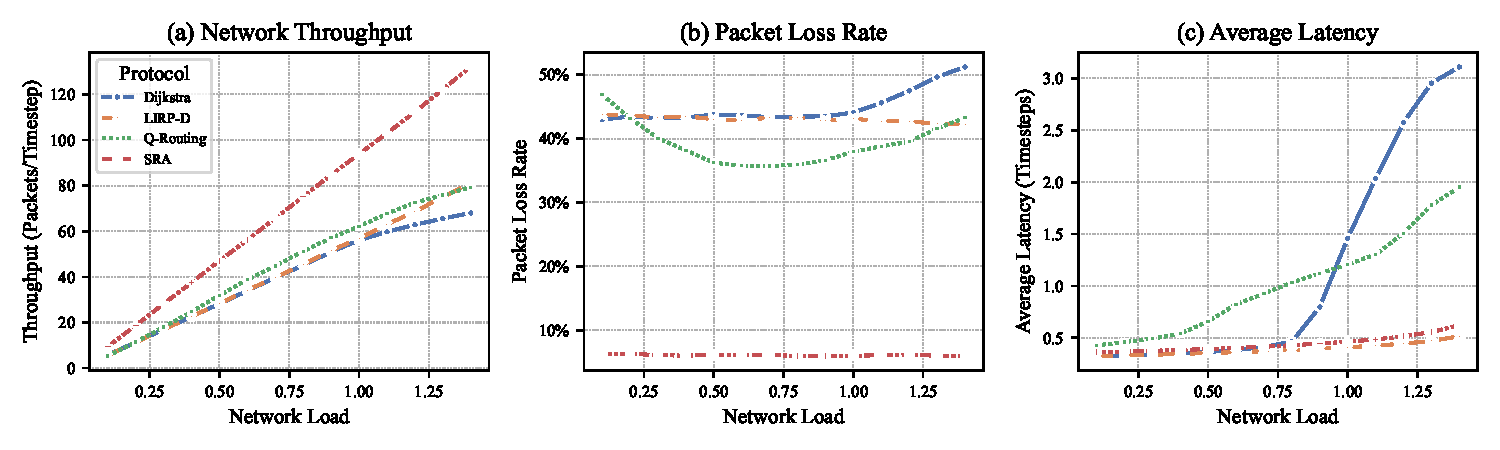
\includegraphics[width=0.95\textwidth]{performance_comparison_ba.pdf}
        \caption{Performance on BA Network. SRA functions as a \textbf{proactive performance optimizer}, achieving significantly higher throughput and lower packet loss in the bottleneck-prone topology} % This empty caption is REQUIRED to generate the "(a)" label
        \label{fig:perf_ba_stacked}
    \end{subfigure}
    
    \vspace{0.5cm}

    % (b) WS Network Plot
    \begin{subfigure}{\textwidth}
        \centering
        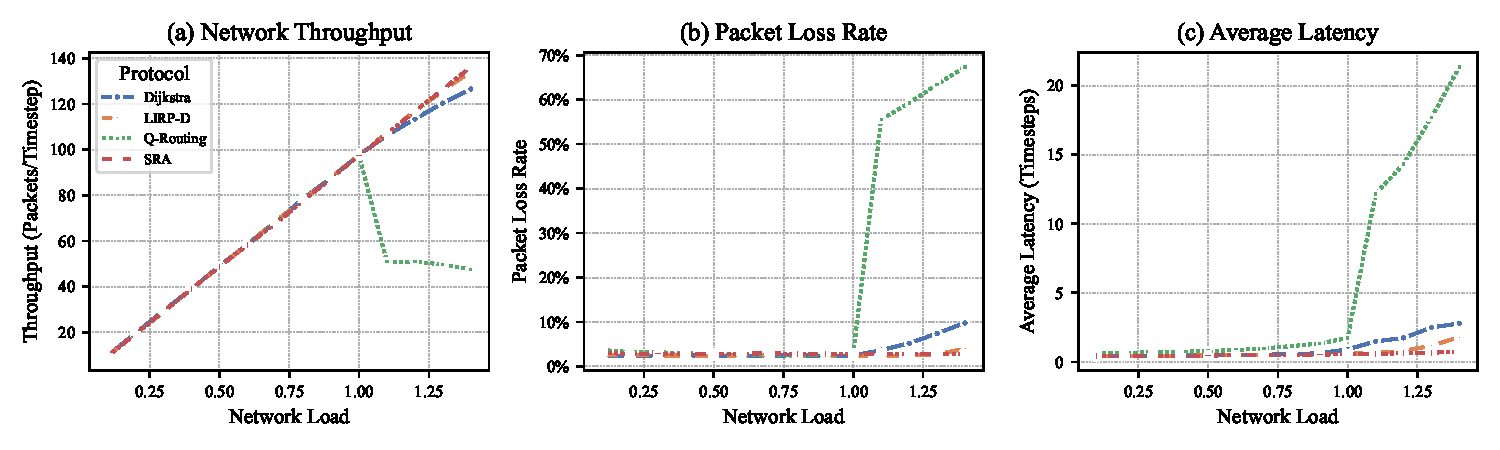
\includegraphics[width=0.95\textwidth]{performance_comparison_ws.pdf}
        \caption{Performance on WS Network. SRA \textbf{showcases its role in guaranteeing stability}, uniquely maintaining performance after the network reaches its critical "congestion knee" (load > 1.0), a point where Q-Routing collapses} % This empty caption is REQUIRED to generate the "(b)" label
        \label{fig:perf_ws_stacked}
    \end{subfigure}

    \vspace{0.5cm}

    % (c) ER Network Plot
    \begin{subfigure}{\textwidth}
        \centering
        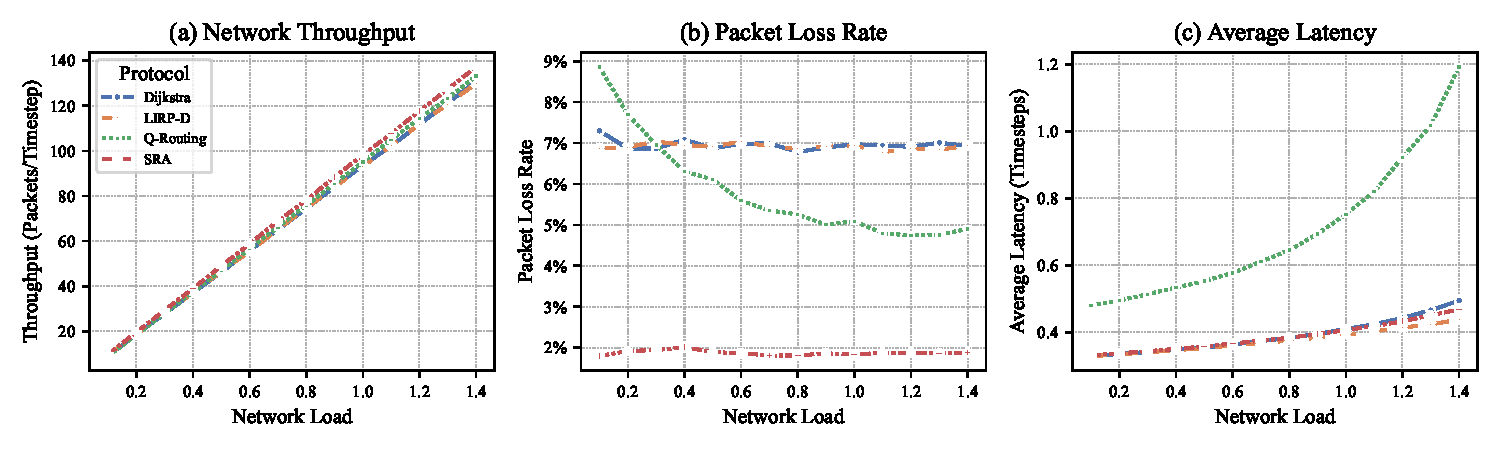
\includegraphics[width=0.95\textwidth]{performance_comparison_er.pdf}
        \caption{Performance on ER Network. SRA functions as a \textbf{resilience enhancement mechanism}, trading a predictably higher latency for a significant reduction in packet loss, thereby enhancing overall reliability} % This empty caption is REQUIRED to generate the "(c)" label
        \label{fig:perf_er_stacked}
    \end{subfigure}
    
    % The main caption for the entire figure collection
    \caption{Dynamic traffic performance comparison of SRA against benchmark protocols across three distinct network topologies. The sub-captions highlight SRA's adaptive, topology-dependent roles.}
    \label{fig:perf_comparison_stacked} % The label for the entire figure
\end{figure*}


The preceding sections have confirmed the SRA algorithm's effectiveness in optimizing the network's stress distribution from the perspectives of static topology and microscopic path selection. This section aims to quantify the actual impact of SRA's structural optimization on key performance indicators (KPIs) under dynamic load, by means of discrete-event traffic simulations. The comprehensive results, presented in Fig.~\ref{fig:perf_comparison_stacked}, reveal that SRA's behavior is highly adaptive, transforming its role based on the network's underlying structure.

\paragraph{Performance on BA Networks (Heterogeneous Topology)}
In the heterogeneous BA network, where performance is constrained by severe structural bottlenecks, SRA demonstrates its profound value as a \textbf{proactive performance optimizer}. The results in Fig.~\ref{fig:perf_comparison_stacked}(a) show that SRA fundamentally alters the network's capacity and reliability. While the throughput of benchmark protocols like Dijkstra, LIRP-D, and Q-Routing saturates quickly around 60-70 packets/timestep, SRA's throughput continues to scale linearly with the load, effectively doubling the network's capacity in high-load scenarios. This performance gain is a direct consequence of its superior congestion management, evidenced by a dramatically lower packet loss rate that remains below 10\%, whereas other protocols suffer catastrophic losses exceeding 40\%. Furthermore, SRA achieves this with controlled latency growth, avoiding the explosion seen in Dijkstra under congestion.

\paragraph{Performance on WS Networks (Hybrid Topology)}
The WS network simulation, presented in Fig.~\ref{fig:perf_comparison_stacked}(b), highlights SRA's crucial role in \textbf{guaranteeing system stability}, especially during network state phase transitions. In the low-load regime (load < 1.0), all protocols perform similarly. However, as the load surpasses the critical "congestion knee," their behaviors diverge dramatically. The learning-based Q-Routing protocol suffers a catastrophic performance collapse. In contrast, SRA is the only protocol that smoothly navigates this critical transition, maintaining stable throughput and controlled packet loss and latency, thus ensuring "graceful degradation" under high stress.

\paragraph{Performance on ER Networks (Homogeneous Topology)}
In the homogeneous ER network, which lacks dominant bottlenecks, SRA intelligently transforms its role into a \textbf{resilience enhancement mechanism}, focusing on reliability. As shown in Fig.~\ref{fig:perf_comparison_stacked}(c), all four protocols exhibit nearly identical throughput performance. However, a significant divergence appears in reliability. While traditional protocols maintain a packet loss rate of around 7\%, SRA consistently suppresses it to a much lower level of approximately 2\%. This reliability enhancement comes at the cost of a higher average latency, showcasing SRA's adaptive "latency-for-reliability" trade-off.




\subsection{Parameter Sensitivity Analysis}
\label{subsec:param_sensitivity}

\begin{figure*}[h!]
    \centering
    % Ensure the path to your PDF file is correct
    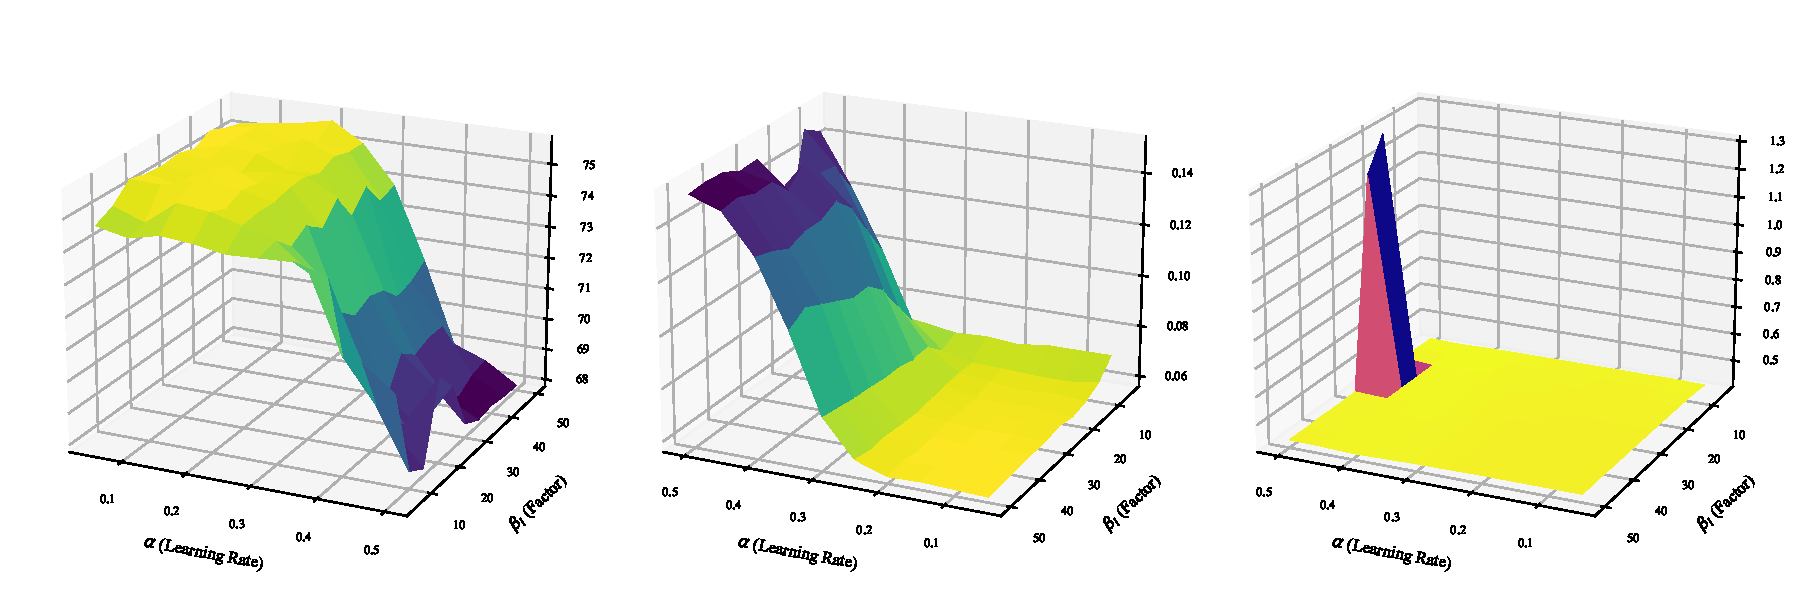
\includegraphics[width=\textwidth]{sensitivity_3d_surfaces_full.pdf}
    \caption{Parameter sensitivity analysis of SRA on a BA network, visualized as 3D surfaces. The plots illustrate the trade-off between (a) maximizing throughput, (b) minimizing packet loss, and (c) minimizing average latency, as a function of the learning rate ($\alpha$) and the pressure-cost factor ($\beta_I$).}
    \label{fig:sensitivity_3d}
\end{figure*}

This section investigates how the SRA core hyperparameters—the learning rate $\alpha$ and the pressure-cost factor $\beta_I$—govern final network performance by analyzing simulations on a BA network under a fixed high load. The 3D surface plots in Fig.~\ref{fig:sensitivity_3d} reveal a classic and critical performance trade-off governed by these parameters.

The results consistently show that parameter choices favoring high throughput and reliability conflict with those that favor low latency. As visualized in Fig.~\ref{fig:sensitivity_3d}(a) and (b), throughput and reliability (i.e., lower packet loss) generally improve with a higher pressure-cost factor ($\beta_I$). This is because a larger $\beta_I$ enforces a more aggressive load-balancing policy, decisively diverting traffic away from high-stress nodes. However, this gain comes at a direct cost to network latency, as shown by the rising surface in Fig.~\ref{fig:sensitivity_3d}(c). A higher $\beta_I$ value controls the "detouring" aggressiveness, forcing packets onto physically longer paths and thus increasing their average transit time.

The data allows us to precisely quantify this trade-off. For instance, the lowest average latency (\textbf{0.422} timesteps) was achieved at $(\alpha=0.45, \beta_I=5.0)$. However, operating at this point resulted in a suboptimal throughput of 71.84 packets/timestep and a high packet loss rate of 9.9\%. Conversely, the lowest packet loss rate (\textbf{5.8\%}) was achieved at a much higher $\beta_I$ of 45.0. This highlights that $\beta_I$ acts as the primary lever for network operators to navigate the trade-off between reliability and speed.

This analysis provides clear guidance for network operators: the SRA parameters allow for a direct trade-off between maximizing \textbf{capacity and reliability} (favored by high $\beta_I$) and optimizing for \textbf{low latency} (favored by low $\beta_I$). For instance, in large-scale data centers where throughput is paramount, higher parameter values should be chosen. Conversely, in real-time applications with stringent delay requirements, $\beta_I$ can be tuned lower.

\subsection{Comprehensive Robustness Analysis: Topology-Dependent Performance Advantages}
\label{subsec:robustness}

To fundamentally quantify the robustness gains provided by SRA and ensure the statistical significance of our findings, we designed a rigorous testing procedure. This procedure was applied to the default BA, WS, and ER network topologies defined in Table~\ref{tab:sim_params}. For each topology, a targeted attack was simulated by sequentially removing nodes in descending order of their initial Betweenness Centrality (BC). After each node removal, we calculated the Packet Delivery Rate (PDR) on the damaged network for both the SRA and Dijkstra policies. PDR is defined as:
\begin{equation}
\label{eq:pdr}
\text{PDR} = \frac{\text{Number of Packets Successfully Received}}{\text{Total Number of Packets Sent}}
\end{equation}
To compare the two policies, we define the SRA PDR Advantage (\%) as the primary metric for our analysis:
\begin{equation}
\label{eq:pdr_advantage}
\text{PDR Advantage (\%)} = \frac{\text{PDR}_{\text{SRA}} - \text{PDR}_{\text{Dijkstra}}}{\text{PDR}_{\text{Dijkstra}}} \times 100\%
\end{equation}
To ensure the results are statistically robust, this entire process was repeated for 50 independent runs, each on a newly generated network instance. The final results, presented in Fig.~\ref{fig:robustness_summary_stats}, show the mean and standard deviation of this advantage metric across all runs.

\begin{figure}[t!]
    \centering
    % Please ensure the file path to your PDF is correct
    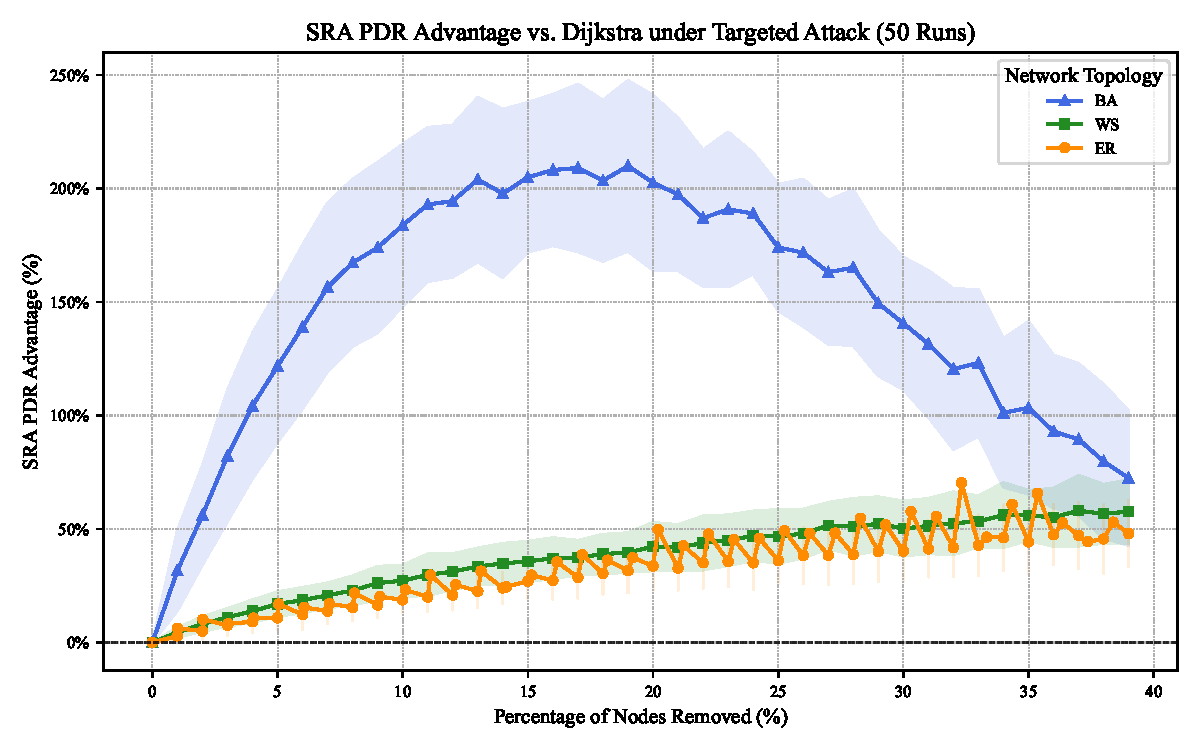
\includegraphics[width=\columnwidth]{robustness_advantage_summary_stats.pdf}
    \caption{The SRA PDR Advantage over the Dijkstra policy under a targeted attack (mean and standard deviation over 50 runs). The solid lines represent the mean advantage, while the shaded areas depict the standard deviation, indicating the consistency of the results.}
    \label{fig:robustness_summary_stats}
\end{figure}

\begin{enumerate}
    \item \textbf{Statistically Confirmed Advantage in BA Networks:} The results for the BA network (blue curve) provide strong statistical validation for SRA's role as a "performance engineer." The mean PDR advantage immediately exceeds \textbf{60\%} even before any attacks, and this significant gain is sustained. Crucially, the extremely narrow standard deviation band indicates that this massive reliability improvement is a \textbf{highly consistent and predictable} outcome across different network instances, not an artifact of a single simulation.

    \item \textbf{Emergent but Variable Advantage in WS Networks:} The WS network (green curve) confirms that SRA's advantage "emerges" when the network is pushed into a critical state, with the mean advantage peaking around \textbf{20\%} after 15\% of nodes are removed. Interestingly, the wider standard deviation band reveals a new insight: while the advantage is significant on average, its magnitude exhibits higher \textbf{variability} compared to other topologies. This suggests that the structural outcome of targeted attacks on WS networks is more diverse, leading to a wider range of performance gains from SRA.

    \item \textbf{Consistently Neutral Performance in ER Networks:} The ER network (orange curve) serves as a powerful control case. The mean advantage remains tightly bound to the \textbf{0\% baseline}, and the narrow deviation band confirms this neutral performance is \textbf{highly consistent}. This is not a failure but a testament to SRA's targeted intelligence: in an already robust topology, it correctly avoids unnecessary interventions.
\end{enumerate}

This statistically robust analysis provides decisive evidence for SRA's \textbf{topology-dependent} nature. It validates that SRA's resilience-enhancing benefits are significant and reliable in networks with structural vulnerabilities (BA), emergent under critical damage (WS), and correctly neutral in inherently robust networks (ER).

\section{Discussion}
\label{sec:discussion}

The extensive simulation results have systematically demonstrated that the System Relaxation Algorithm (SRA) not only effectively disperses structural stress but also translates this optimization into measurable, context-dependent performance gains. This Section provides an in-depth interpretation of these findings, dissecting the core trade-offs that SRA navigates and clarifying the decisive role of network topology.

\subsection{The Core Trade-off: Topology-Dependent Performance and Resilience}

The central value of SRA lies not in the cost-free optimization of a single metric, but in its intelligent, topology-aware navigation of the fundamental trade-off between \textbf{performance and resilience}. Our results reveal that SRA acts as an adaptive controller, dynamically choosing its optimization strategy based on the network's structural characteristics.

In \textbf{heterogeneous networks} like the BA model, where performance is inherently limited by structural bottlenecks, SRA prioritizes maximizing performance. It willingly sacrifices a minor degree of path efficiency---a mere \textbf{7.80\%} increase in average path length---in exchange for a massive gain in network capacity and reliability. This structural overhaul, evidenced by an \textbf{80.18\%} reduction in peak centrality, transforms SRA into a \textbf{proactive performance optimizer}, fundamentally elevating the operational ceiling of structurally fragile networks.

Conversely, in \textbf{homogeneous networks} like the ER and WS models, which lack dominant bottlenecks, SRA's strategy shifts to enhancing resilience. Recognizing that the network's capacity is not the primary constraint, SRA acts as a "risk manager." It makes finer adjustments to proactively manage both dynamic congestion risks (reducing packet loss from 7\% to 2\% in ER networks) and structural damage risks (providing a PDR advantage of nearly 20\% in critically damaged WS networks). This proves that SRA's equilibrium is not a one-size-fits-all solution, but a sophisticated, multi-dimensional decision that intelligently balances efficiency, performance, and resilience according to the specific needs of the topology.

\subsection{The Nature of SRA's Dynamic Equilibrium}

A consistent observation across all simulations is that SRA converges not to a fragile, static fixed point, but to a \textbf{robust and stable attracting set} characterized by bounded fluctuations. This is not a failure of convergence but a profound feature of the system's healthy, adaptive state. This dynamic equilibrium stems from two intrinsic properties: the \textbf{non-smoothness} of path selection, where a marginal cost change can trigger a discrete "jump" in routing policy, and the inherent \textbf{feedback latency} of the global system.

SRA's core mechanism, the "leaky integrator," is precisely designed to manage this dynamic. The integral term provides "memory" to suppress violent oscillations, while the decay term acts as a powerful "damping" force that continuously dissipates system energy. The result, as theoretically proven by our piecewise Lyapunov analysis and empirically validated in Fig.~\ref{fig:lyapunov_dynamics} and Fig.~\ref{fig:dwell_time_effect}, is a predictable and bounded dynamic behavior---a living equilibrium that is far more resilient to real-world perturbations than a static optimum would be.

\subsection{Positioning in Modern Architectures and Future Outlook}

Positioned within modern network architectures, SRA is not a competitor to Software-Defined Networking (SDN) but rather a powerful, model-driven application designed to run on an SDN controller. The SDN paradigm resolves one of the main challenges for SRA's practical deployment: the computational cost of centrality analysis. An SDN controller's inherent global view makes the collection of network-wide topology information trivial, turning the computationally intensive stress analysis into a practically feasible task for a centralized entity.

In this context, SRA provides the missing "control logic" that enables an SDN controller to move beyond simple connectivity management towards intelligent, proactive stress governance. This paper lays a theoretical foundation for such model-driven resilient networks and opens several exciting directions for future research. Key among them are: 1) integrating the SRA framework with mainstream SDN controllers (e.g., ONOS or Ryu) and designing efficient Northbound APIs; 2) validating the framework on real-world data from Internet AS topologies or data centers; and 3) exploring adaptive parameter tuning mechanisms to achieve an even higher order of self-organization.


\section{Conclusion}
\label{sec:conclusion}

In response to the "stress concentration" problem endemic to conventional network control paradigms, this paper introduced, analyzed, and validated the System Relaxation Algorithm (SRA). We established the SRA framework on a rigorous theoretical foundation, uniquely applying the theory of non-smooth dynamical systems to formally prove the stability of a system managing discontinuous path-switching dynamics. Comprehensive simulations then decisively demonstrated SRA's core value: its profound, topology-dependent intelligence. The results show SRA adaptively functions as a proactive performance optimizer in bottleneck-prone heterogeneous networks, while shifting its role to a resilience enhancement mechanism in more homogeneous ones. Ultimately, SRA represents an interpretable and predictable paradigm for designing self-organizing network control strategies that achieve a targeted, intelligent trade-off between performance and resilience, laying a solid foundation for future network governance.


% --- REFERENCES ---
% Use a bibtex file (.bib) is recommended for easier management.
% However, if you prefer to manually format it, here is the thebibliography environment.

\bibliographystyle{IEEEtran}
\bibliography{references}

% The \appendix command switches the section numbering to letters (A, B, C...)

\appendices
\section{Proof of Lemma \ref{lemma:invariance}}
\label{app:proof_lemma_invariance}
\begin{IEEEproof}
\textit{(a) Positive Invariance:}
Take any $S^{(k)}\in X$. By max-value normalization, $\mathcal N(S^{(k)})\subset[0,1]^N=X$. For any choice of $c^{(k)}\in\mathcal N(S^{(k)})$ and any coordinate $i$, we have
\begin{equation}
S^{(k+1)}_i=(1-\alpha)S^{(k)}_i+\alpha\,c^{(k)}_i,
\quad\text{where}\quad S^{(k)}_i,c^{(k)}_i\in[0,1].
\end{equation}
Thus,
\begin{equation}
0\cdot(1-\alpha)+0\cdot\alpha\ \le\ S^{(k+1)}_i\ \le\ 1\cdot(1-\alpha)+1\cdot\alpha,
\end{equation}
which implies $S^{(k+1)}_i\in[0,1]$. As this holds for each coordinate, $S^{(k+1)}\in X$. This shows that $F(X)\subset X$: \textbf{if the state is in $X$ at the current step, it remains in $X$ at the next step}. Therefore, $X$ is a positively invariant set.

\textit{(b) Compactness:}
The set $X=[0,1]^N$ is a closed and bounded hypercube, and is therefore compact.

\textit{(c) Absorbing Property on the "Effective State Space":}
The algorithm and analysis in this paper are initialized within $X$ ($S^{(0)}\in X$), and from (a), we know $F(X)\subset X$. Therefore, for the discrete-time semi-flow on the state space $X$,
\begin{equation}
\Phi(k,\cdot):X\to 2^X,\quad \Phi(1,\cdot)=F,\ \ \Phi(k+1,\cdot)=F\circ\Phi(k,\cdot),
\end{equation}
the set $X$ \textbf{absorbs itself}: for any bounded set $B\subset X$, choosing $n_B=0$ yields $\Phi(n,B)\subset X$ for all $n\ge 0$. By standard definitions, this means \textbf{$X$ is a compact absorbing set}.

\textit{(d) (Optional supplement for stability intuition):}
If we permit an initial value $S^{(0)}\notin X$, we can still show \textbf{exponential attraction} to $X$. Define the "out-of-bounds quantity" for any coordinate as
\begin{equation}
\delta^+_{k,i}:=\max\{S^{(k)}_i-1,\,0\},\qquad 
\delta^-_{k,i}:=\max\{-S^{(k)}_i,\,0\}.
\end{equation}
Since $c^{(k)}_i\in[0,1]$, we have
\begin{equation}
\begin{aligned}
S^{(k+1)}_i-1 &= (1-\alpha)(S^{(k)}_i-1)+\alpha(c^{(k)}_i-1)\ \le\ (1-\alpha)(S^{(k)}_i-1),\\
-S^{(k+1)}_i &\le\ (1-\alpha)(-S^{(k)}_i).
\end{aligned}
\end{equation}


This leads to
\begin{equation}
\delta^+_{k+1,i}\ \le\ (1-\alpha)\,\delta^+_{k,i},\qquad 
\delta^-_{k+1,i}\ \le\ (1-\alpha)\,\delta^-_{k,i}.
\end{equation}
This means that $\max\{\delta^+_{k,i},\delta^-_{k,i}\}$ converges geometrically to 0 at a rate of $1-\alpha$, and thus $\mathrm{dist}_\infty(S^{(k)},X)\le (1-\alpha)^k\,\mathrm{dist}_\infty(S^{(0)},X)\to0$. This shows \textbf{exponential attraction} to $X$. The main procedure of this paper is initialized within $X$, so the absorbing set formulation in (c) is sufficient.

In conclusion, $X=[0,1]^N$ is positively invariant and compact for the system, and it is a compact absorbing set on the discrete-time semi-flow with state space $X$.
\end{IEEEproof}

\section{Proof of Proposition \ref{prop:usc}}
\label{app:proof_prop_usc}
\begin{IEEEproof}
\textit{(a) Non-empty, Compact, and Convex Values:}
By the definitions in Sections 3.1--3.2, $\mathrm{norm}(\kappa(S))\in[0,1]^N$. Thus, for any $S$,
\begin{equation}
\mathcal N(S)=\mathrm{co}\!\big(\mathrm{norm}(\kappa(S))\big)\subset[0,1]^N.
\end{equation}
The closed convex hull, $\mathrm{co}(\cdot)$, of a non-empty set is \textbf{non-empty}. It is also a \textbf{closed and bounded} convex subset of $[0,1]^N$, and is therefore \textbf{compact} and \textbf{convex}.

\textit{(b) Piecewise Constant Structure and Finiteness:}
The graph $G$ and the set of source-destination (OD) pairs are finite. The node cost $C(S)$ is an affine function of $S$. For each OD pair $(s,t)$, the set of candidate simple paths is \textbf{finite}. The cost of each path is the \textbf{pointwise minimum} of a family of affine functions of $S$. Thus, there exists a \textbf{finite partition} of the state space of $S$ such that within each partition, the set of shortest paths for every OD pair remains \textbf{constant}. Therefore, within each partition, $\kappa(S)$ and $\mathrm{norm}(\kappa(S))$ are \textbf{constant vectors}. On the boundaries of these partitions, the limit of $\mathrm{norm}(\kappa(S))$ can only be one of the constant values from the \textbf{finite set of adjacent partitions}. Let these constant vectors be $\{v_\ell\}_{\ell\in\mathcal I(S)}$, where $\mathcal I(S)$ is the finite index set of partitions adjacent to $S$. Then,
\begin{equation}
\mathcal N(S)=\mathrm{co}\big(\{v_\ell:\,\ell\in\mathcal I(S)\}\big).
\end{equation}
This establishes the structure of $\mathcal N(\cdot)$ as being \textbf{piecewise constant with the closed convex hull taken at the boundaries}.

\textit{(c) Upper Semi-Continuity (USC) via Sequential Criterion / Closed Graph:}
Take an arbitrary sequence $S_n\to S$, and let $c_n\in\mathcal N(S_n)$ such that $c_n\to c$. We must show that $c\in\mathcal N(S)$. From (b), for each $n$, there exists a finite set $\{v_{\ell}: \ell\in\mathcal I(S_n)\}$ such that $c_n\in\mathrm{co}\big(\{v_{\ell}:\ell\in\mathcal I(S_n)\}\big)$. By Carathéodory's theorem, we can write
\begin{equation}
c_n=\sum_{j=0}^{N} \lambda_{n,j}\, v_{\ell_{n,j}},\quad 
\lambda_{n,j}\ge 0,\ \sum_{j=0}^{N}\lambda_{n,j}=1,\ 
\ell_{n,j}\in\mathcal I(S_n).
\end{equation}
Since the vectors $v_{\ell}$ come from a \textbf{globally finite} set $\{v_1,\dots,v_M\}$, we can pass to a subsequence to ensure $\ell_{n,j}\equiv \bar\ell_j$ is \textbf{fixed}, and (by compactness of $[0,1]$) $\lambda_{n,j}\to \bar\lambda_j$. Then,
\begin{equation}
c=\lim_{n\to\infty} c_n=\sum_{j=0}^{N}\bar\lambda_j\, v_{\bar\ell_j},
\quad\sum_{j=0}^{N}\bar\lambda_j=1,\ \bar\lambda_j\ge 0.
\end{equation}
Since $S_n\to S$, for $n$ large enough, any limit index $\bar\ell_j$ must belong to $\mathcal I(S)$. Thus, each limit vector $v_{\bar\ell_j}$ is one of the constant vectors from a partition adjacent to $S$. Therefore,
\begin{equation}
c=\sum_{j=0}^{N}\bar\lambda_j\, v_{\bar\ell_j}\ \in\ 
\mathrm{co}\big(\{v_\ell:\,\ell\in\mathcal I(S)\}\big)=\mathcal N(S).
\end{equation}
This means the graph of $\mathcal N$, $\mathrm{gph}\,\mathcal N:=\{(S,c):\,c\in\mathcal N(S)\}$, is closed. A closed-graph map with compact values is \textbf{USC}.

\textit{(d) Properties of $F(\cdot)$:}
Scaling and translation preserve the USC property and non-empty, compact, convex values. The map $S\mapsto (1-\alpha)S$ is continuous (single-valued). The Minkowski sum $F(S)=(1-\alpha)S+\alpha\,\mathcal N(S)$ of a continuous map and a USC map is also USC with non-empty, compact, and convex values.
\end{IEEEproof}

\section{Proof of Theorem \ref{thm:attractor}}
\label{app:proof_thm_attractor}
\begin{IEEEproof}
\textit{(a) Pre-compactness:}
From Lemma \ref{lemma:invariance}, $X=[0,1]^N$ is a compact, positively invariant set. Thus, any trajectory starting in $X$ remains in $X$. Since $X$ is compact, any trajectory is \textbf{pre-compact} (i.e., has a convergent subsequence).

\textit{(b) Existence of $\omega$-limit sets:}
For any $S^{(0)}\in X$, its $\omega$-limit set is defined as
\begin{equation}
\omega\big(S^{(0)}\big)\ :=\ \left\{x\in X:\ \exists\,k_n\uparrow\infty\ \text{s.t.}\ S^{(k_n)}\to x\right\}.
\end{equation}
By pre-compactness, $\omega(S^{(0)})$ is \textbf{non-empty} and \textbf{compact}.

\textit{(c) Positive Invariance of $\omega$-limit sets:}
From Proposition \ref{prop:usc}, $F(\cdot)$ is USC with compact values, which implies its graph is closed. Take any $x \in \omega(S^{(0)})$. By definition, there is a subsequence $S^{(k_n)} \to x$. The subsequent points $S^{(k_n+1)} \in F(S^{(k_n)})$ are in the compact set $X$, so a further subsequence converges, $S^{(k_n+1)} \to y$. By the closed graph property, $y \in F(x)$. Since $\{k_n+1\}$ also tends to infinity, $y$ is also in $\omega(S^{(0)})$. Thus,
\begin{equation}
F\big(\omega(S^{(0)})\big)\ \subset\ \omega(S^{(0)}).
\end{equation}

\textit{(d) Attraction to $\omega$-limit sets:}
It can be shown by contradiction that the trajectory must approach its $\omega$-limit set. Thus, $\mathrm{dist}\big(S^{(k)},\omega(S^{(0)})\big)\ \to\ 0$.

\textit{(e) Global Attractor:}
Let $\Omega$ be the union of all $\omega$-limit sets for all starting points in $X$:
\begin{equation}
\Omega\ :=\ \bigcup_{S^{(0)}\in X} \omega(S^{(0)}).
\end{equation}
This set $\Omega$ is non-empty, compact, and positively invariant. For any $S^{(0)}\in X$, since $\mathrm{dist}(S^{(k)},\omega(S^{(0)}))\to 0$ and $\omega(S^{(0)})\subset\Omega$, it follows that
\begin{equation}
\mathrm{dist}\big(S^{(k)},\Omega\big)\ \to\ 0.
\end{equation}
Thus, $\Omega$ is a global attractor for the system.
\end{IEEEproof}

\section{Proof of Theorem \ref{thm:drop_jump}}
\label{app:proof_thm_drop_jump}
\begin{IEEEproof}
Let $c_k\in\arg\min_{c\in\mathcal N(S^{(k)})}\|S^{(k)}-c\|_2^2$, so $V(S^{(k)})=\|S^{(k)}-c_k\|_2^2$.
From the discrete-time inclusion, let $S^{(k+1)}=(1-\alpha)S^{(k)}+\alpha\,c_k$.
Let $c_{k+1}\in\mathcal N(S^{(k+1)})$ be a minimizer for $V(S^{(k+1)})$. We can write
\begin{equation}
S^{(k+1)}-c_{k+1}=(1-\alpha)(S^{(k)}-c_k) + (c_k-c_{k+1}).
\end{equation}
Using the Weighted Young's Inequality $\|x+y\|_2^2\le (1+\lambda)\|x\|_2^2+(1+1/\lambda)\|y\|_2^2$ with $\lambda=\alpha/(1-\alpha)$, we get
\begin{equation}
\|S^{(k+1)}-c_{k+1}\|_2^2 \le (1-\alpha)\|S^{(k)}-c_k\|_2^2 + \frac{1}{\alpha}\,\|c_k-c_{k+1}\|_2^2.
\end{equation}
Since $c_k$ and $c_{k+1}$ belong to the convex hull of a finite set of vectors, the distance between them is bounded, $\|c_k-c_{k+1}\|\le \bar\Delta$. Substituting this in gives the desired inequality. The limit superior result follows from solving the linear recurrence inequality.
\end{IEEEproof}

\section{Proof of Corollary \ref{cor:local_convergence}}
\label{app:proof_cor_local_convergence}
\begin{IEEEproof}
(1) \textbf{Uniqueness of Fixed Point:} Solving $S=(1-\alpha)S+\alpha c$ gives $\alpha S=\alpha c$, so $S=c$. The unique fixed point is $S^\star=c$.
(2) \textbf{Contraction and Convergence Rate:}
\begin{equation}
S^{(k+1)}-c = (1-\alpha)S^{(k)}+\alpha c-c = (1-\alpha)\big(S^{(k)}-c\big).
\end{equation}
Taking the 2-norm and iterating gives the result:
\begin{equation}
\|S^{(k)}-S^\star\|_2 = (1-\alpha)^k\,\|S^{(0)}-S^\star\|_2.
\end{equation}
\end{IEEEproof}

\section{Proof of Proposition \ref{prop:block_dynamics}}
\label{app:proof_prop_block_dynamics}
\begin{IEEEproof}
(i) Within a block, $\mathcal N(S)\equiv\{c_m\}$ is constant. The "jump" term in the inequality of Theorem \ref{thm:drop_jump} is zero. So, $V_{k+1}\le \gamma V_k$, and iterating this $t$ times gives the result.
(ii) At the boundary between block $m$ and $m+1$, a switch is allowed. We apply the "drop-jump" inequality for this single step:
\begin{equation}
\begin{split}
V_{m+1} = V(S^{(\tau_{m+1})}) & \le \gamma\,V(S^{(\tau_{m+1}-1)}) + \tilde C \\
& = \gamma\,V(S^{(\tau_m+T_d-1)}) + \tilde C \\
& \le \gamma \cdot (\gamma^{T_d-1}V_m) + \tilde C = \gamma^{T_d}V_m + \tilde C,
\end{split}
\end{equation}
where the last inequality uses the result from (i).
\end{IEEEproof}

\section{Proof of Theorem \ref{thm:epsilon_tube}}
\label{app:proof_thm_epsilon_tube}
\begin{IEEEproof}
(a) Iteratively expanding the linear recurrence from Proposition \ref{prop:block_dynamics}(ii), $V_{m+1}\le \gamma^{T_d}V_m+\tilde C$, gives:
\begin{equation}
\begin{split}
V_m &\le (\gamma^{T_d})^m V_0 + \tilde C \sum_{j=0}^{m-1}(\gamma^{T_d})^j \\
    &= \gamma^{mT_d}V_0 + \tilde C\,\frac{1-\gamma^{mT_d}}{1-\gamma^{T_d}} \\
    &\le \gamma^{mT_d}V_0+\frac{\tilde C}{1-\gamma^{T_d}}.
\end{split}
\end{equation}
Taking the limit superior as $m\to\infty$ gives the steady-state radius.
(b) Setting $V_m\le \varepsilon^2$ and solving for $m$ using the upper bound from (a) gives the result.
\end{IEEEproof}

\section{Proof of Theorem \ref{thm:practical_stability}}
\label{app:proof_thm_practical_stability}
\begin{IEEEproof}
(a) By definition of the minimum dwell time, after a switch, no other switch is permitted for at least $T_d$ steps. Thus, the number of switches in a window of length $T$ is bounded.
(b) This result is a direct consequence of solving the inter-block recurrence, as shown in the proof of Theorem \ref{thm:epsilon_tube}(a).
(c) This result follows from inverting the inequality in Theorem \ref{thm:epsilon_tube}(b).
\end{IEEEproof}

% --- START: New Appendices for Section III-E ---

\section{Proof of Lemma~\ref{lem:block-budget}}
\label{app:proof_lem_block_budget}
\begin{IEEEproof}
The proof consists of two parts: bounding the non-peak increase and guaranteeing the peak decrease.

\noindent\textit{1) Bounding Non-Peak Increase:}
Let $c^{(m)}$ and $c^{(m+1)}$ be the normalized centrality vectors at the start and end of the block. By definition of $\bar\Delta$, we have $\|c^{(m+1)}-c^{(m)}\|_\infty \le \bar\Delta$, which means $|c^{(m+1)}_j - c^{(m)}_j| \le \bar\Delta$ for all $j$.
The unnormalized centralities are $\kappa^{(m)}_j = c^{(m)}_j \kappa^{(m)}_{\max}$ and $\kappa^{(m+1)}_j = c^{(m+1)}_j \kappa^{(m+1)}_{\max}$.
Since the peak centrality does not increase (and in fact decreases, as shown next), we have $\kappa^{(m+1)}_{\max} \le \kappa^{(m)}_{\max}$.
Therefore, for any non-peak node $j \neq u$:

\begin{align*}
\kappa^{(m+1)}_j - \kappa^{(m)}_j &= c^{(m+1)}_j \kappa^{(m+1)}_{\max} - c^{(m)}_j \kappa^{(m)}_{\max} \\
&\le c^{(m+1)}_j \kappa^{(m)}_{\max} - c^{(m)}_j \kappa^{(m)}_{\max} \\
&= (c^{(m+1)}_j - c^{(m)}_j) \kappa^{(m)}_{\max} \\
&\le |c^{(m+1)}_j - c^{(m)}_j| \kappa^{(m)}_{\max} \le \bar\Delta \cdot \kappa^{(m)}_{\max} =: B^{(m)}.
\end{align*}

\noindent\textit{2) Guaranteeing Peak Decrease ($\delta>0$):}
The existence of a net peak decrease is a direct consequence of the system dynamics proven in Section~\ref{sec:convergence_analysis}. The drop-jump inequality (Theorem~\ref{thm:drop_jump}) and the dwell-time policy (Theorem~\ref{thm:practical_stability}) guarantee that the system does not reach a fixed point but evolves within a stable attractor, forcing state transitions.
A state transition (path switch) is triggered when the cost of a high-centrality node $u$, $C_u = 1 + \beta_I S_u$, increases sufficiently to make an alternative path cheaper. The state update rule $S_u^{(k+1)} = (1-\alpha)S_u^{(k)} + \alpha c_u^{(k)}$ ensures that a node with peak normalized centrality ($c_u=1$) experiences the strongest pressure increase.
This mechanism guarantees that traffic is eventually diverted from the peak node $u$. As the network is assumed to have no structurally unavoidable bottlenecks, this diversion must lead to a strict reduction in its unnormalized centrality, $\kappa_u$. Therefore, there must exist a net decrease $\delta > 0$ over any block that contains such a path-switching event. The magnitude of $\delta$ depends on the system parameters ($\alpha, \beta_I, T_d$) and the network topology, but its existence is guaranteed by the convergence dynamics.
\end{IEEEproof}

\section{Proof of Proposition~\ref{prop:perf-bridge}}
\label{app:proof_prop_perf_bridge}
\begin{IEEEproof}
The proof leverages the guaranteed peak reduction $\kappa'_{\max} < \kappa_{\max}$ established in Lemma~\ref{lem:block-budget}.

\noindent\textit{(i) Unconditional robust lower bound:}
The robust lower bound on capacity is defined as $L(\kappa) := \mu_{\min}/\kappa_{\max}$.
Since SRA does not change the physical node service rates, $\mu_{\min}$ is a constant.
Given that $\kappa'_{\max} < \kappa_{\max}$, it follows directly that:
\begin{equation}
L(\kappa') = \frac{\mu_{\min}}{\kappa'_{\max}} > \frac{\mu_{\min}}{\kappa_{\max}} = L(\kappa).
\end{equation}
The lower bound strictly increases.

\noindent\textit{(ii) Aligned-bottleneck capacity gain:}
The network capacity is defined as $\rho_{\max}(\kappa) = \min_{i \in V} \frac{\mu_i}{\kappa_i}$.
The new capacity after SRA is $\rho_{\max}(\kappa') = \min_{i \in V} \frac{\mu_i}{\kappa'_i}$.
By definition, the minimum of a set is less than or equal to any individual element. Therefore, the new capacity is lower-bounded by the capacity of the original peak node, $u$:
\begin{equation}
\rho_{\max}(\kappa') \ge \frac{\mu_u}{\kappa'_u}.
\end{equation}
Furthermore, since $u$ may not be the peak node in the new state $\kappa'$, its centrality $\kappa'_u$ must be less than or equal to the new maximum centrality, $\kappa'_{\max}$. Thus:
\begin{equation}
\rho_{\max}(\kappa') \ge \frac{\mu_u}{\kappa'_u} \ge \frac{\mu_u}{\kappa'_{\max}}.
\end{equation}
The premise of this case is that the original bottleneck was at the peak node, so $\rho_{\max}(\kappa) = \mu_u/\kappa_{\max}$. Combining these gives:
\begin{equation}
\rho_{\max}(\kappa') \ge \frac{\mu_u}{\kappa'_{\max}} > \frac{\mu_u}{\kappa_{\max}} = \rho_{\max}(\kappa).
\end{equation}
This proves a strict increase in the actual network capacity.
\end{IEEEproof}

\section{Proof of Theorem~\ref{thm:sufficient-noC2}}
\label{app:proof_thm_sufficient_noC2}
\begin{IEEEproof}
The goal is to show that under the given conditions, the new network capacity $\rho_{\max}^{(m+1)}$ is no less than the original capacity $\rho_{\max}^{(m)}$.
Let $\rho_{\max}^{(m)} = \mu_{i^\star}/\kappa^{(m)}_{i^\star}$, where $i^\star$ is the bottleneck node at the start of the block.
The new capacity is $\rho_{\max}^{(m+1)} = \min_i \frac{\mu_i}{\kappa^{(m+1)}_i}$.

From Lemma~\ref{lem:block-budget}, we have established worst-case bounds on the centrality changes for the peak node $u$ and all non-peak nodes $j \neq u$:
\begin{itemize}
    \item $\kappa^{(m+1)}_u \le \kappa^{(m)}_{\max} - \delta$
    \item $\kappa^{(m+1)}_j \le \kappa^{(m)}_j + B^{(m)}$ for $j \neq u$.
\end{itemize}
This implies that the capacity of each node after the update, $\mu_i / \kappa^{(m+1)}_i$, has a lower bound:
\begin{itemize}
    \item For the peak node $u$: $\frac{\mu_u}{\kappa^{(m+1)}_u} \ge \frac{\mu_u}{\kappa^{(m)}_{\max} - \delta}$
    \item For any non-peak node $j \neq u$: $\frac{\mu_j}{\kappa^{(m+1)}_j} \ge \frac{\mu_j}{\kappa^{(m)}_j + B^{(m)}}$
\end{itemize}
The new network capacity, being the minimum of all individual node capacities, must be greater than or equal to the minimum of these lower bounds:
\begin{equation}
\rho_{\max}^{(m+1)} = \min_i \frac{\mu_i}{\kappa^{(m+1)}_i} \ge \min \! \left\{ \frac{\mu_u}{\kappa^{(m)}_{\max} - \delta}, \min_{j \neq u} \frac{\mu_j}{\kappa^{(m)}_j + B^{(m)}} \right\}.
\end{equation}
The theorem states two sufficient conditions.
\begin{itemize}
    \item If the first condition holds, $\frac{\mu_u}{\kappa^{(m)}_{\max}-\delta} \ge \rho_{\max}^{(m)}$, this means that even after the worst-case evolution, the original peak node's capacity is still no less than the original network capacity.
    \item If the second condition holds, $\forall j: \frac{\mu_j}{\kappa^{(m)}_{j}+B^{(m)}} \ge \rho_{\max}^{(m)}$, this means that even after the worst-case increase in load, no non-peak node becomes a new bottleneck with capacity lower than the original.
\end{itemize}
If either of these conditions is met, the minimum of the lower bounds must be greater than or equal to $\rho_{\max}^{(m)}$. Therefore, $\rho_{\max}^{(m+1)} \ge \rho_{\max}^{(m)}$, which completes the proof.
\end{IEEEproof}



\end{document}